% Template for Elsevier CRC journal article
% version 1.2 dated 09 May 2011

% This file (c) 2009-2011 Elsevier Ltd.  Modifications may be freely made,
% provided the edited file is saved under a different name

% This file contains modifications for Procedia Computer Science

% Changes since version 1.1
% - added "procedia" option compliant with ecrc.sty version 1.2a
%   (makes the layout approximately the same as the Word CRC template)
% - added example for generating copyright line in abstract

%-----------------------------------------------------------------------------------

%% This template uses the elsarticle.cls document class and the extension package ecrc.sty
%% For full documentation on usage of elsarticle.cls, consult the documentation "elsdoc.pdf"
%% Further resources available at http://www.elsevier.com/latex

%-----------------------------------------------------------------------------------

%%%%%%%%%%%%%%%%%%%%%%%%%%%%%%%%%%%%%%%%%%%%%%%%%%%%%%%%%%%%%%
%%%%%%%%%%%%%%%%%%%%%%%%%%%%%%%%%%%%%%%%%%%%%%%%%%%%%%%%%%%%%%
%%                                                          %%
%% Important note on usage                                  %%
%% -----------------------                                  %%
%% This file should normally be compiled with PDFLaTeX      %%
%% Using standard LaTeX should work but may produce clashes %%
%%                                                          %%
%%%%%%%%%%%%%%%%%%%%%%%%%%%%%%%%%%%%%%%%%%%%%%%%%%%%%%%%%%%%%%
%%%%%%%%%%%%%%%%%%%%%%%%%%%%%%%%%%%%%%%%%%%%%%%%%%%%%%%%%%%%%%

%% The '3p' and 'times' class options of elsarticle are used for Elsevier CRC
%% The 'procedia' option causes ecrc to approximate to the Word template
\documentclass[3p,times,procedia]{elsarticle}
\flushbottom

%% The `ecrc' package must be called to make the CRC functionality available
\usepackage{ecrc}
\usepackage[utf8]{inputenc}
\usepackage{amssymb}
\usepackage{multicol}
\usepackage[table,xcdraw]{xcolor}
\usepackage{graphicx}
\usepackage{cellspace}
\usepackage{longtable}
\usepackage{tipa}
\usepackage{amsmath}
\usepackage{amsfonts}
\usepackage{pdfpages}
\usepackage{footnote}
\usepackage{amsthm}
\usepackage{rotating}
\usepackage{multirow}
\usepackage[justification=justified, format=plain]{caption}
\usepackage{relsize}
\usepackage[bookmarks=false]{hyperref}
    \hypersetup{colorlinks,
      linkcolor=blue,
      citecolor=blue,
      urlcolor=blue}
\usepackage{url}
\urlstyle{same}  % Use same font as text for URLs
\usepackage{pifont}
%\usepackage[ruled,vlined,linesnumbered]{algorithm2e}  %nofillcomment, noend
\usepackage{etoolbox}
\usepackage{lipsum}% just to generate some text
\usepackage[english]{babel}
\usepackage[T1]{fontenc}
\usepackage{wrapfig, blindtext}
\usepackage{stackengine}
\usepackage{tabulary}
\usepackage{url}
% \usepackage[noadjust]{cite}  % Conflicts with natbib already loaded by elsarticle
\usepackage{amstext}
\usepackage{array,times}
\usepackage{booktabs,chemformula}
\usepackage[cal=boondox]{mathalfa}
\usepackage[mathscr]{eucal}
\usepackage[newcommands]{ragged2e}
\usepackage{bm}
% \usepackage{cite}  % Conflicts with natbib already loaded by elsarticle
\usepackage{amsmath,amssymb,amsfonts,bm}
\usepackage{float}      % Required for [H] option
\usepackage{placeins}   % Required for \FloatBarrier
% \usepackage{caption}    % Already loaded above with options
\usepackage{booktabs}
\usepackage{tabularx} % For the tabularx environment
\usepackage{algorithm}
\usepackage{algpseudocode}
\usepackage{array}  % Improve table formatting
\usepackage{textcomp}
\usepackage{adjustbox}
\usepackage{verbatim}
\usepackage{listings}
\def\BibTeX{{\rm B\kern-.05em{\sc i\kern-.025em b}\kern-.08em
T\kern-.1667em\lower.7ex\hbox{E}\kern-.125emX}}

%% The ecrc package defines commands needed for running heads and logos.
%% For running heads, you can set the journal name, the volume, the starting page and the authors

%% set the volume if you know. Otherwise `00'
\volume{00}

%% set the starting page if not 1
\firstpage{1}

%% Give the name of the journal
\journalname{Procedia Computer Science}

%% Give the author list to appear in the running head
%% Example \runauth{C.V. Radhakrishnan et al.}
\runauth{Author name}

%% The choice of journal logo is determined by the \jid and \jnltitlelogo commands.
%% A user-supplied logo with the name <\jid>logo.pdf will be inserted if present.
%% e.g. if \jid{yspmi} the system will look for a file yspmilogo.pdf
%% Otherwise the content of \jnltitlelogo will be set between horizontal lines as a default logo

%% Give the abbreviation of the Journal.
\jid{procs}

%% Give a short journal name for the dummy logo (if needed)
%\jnltitlelogo{Computer Science}

%% Hereafter the template follows `elsarticle'.
%% For more details see the existing template files elsarticle-template-harv.tex and elsarticle-template-num.tex.

%% Elsevier CRC generally uses a numbered reference style
%% For this, the conventions of elsarticle-template-num.tex should be followed (included below)
%% If using BibTeX, use the style file elsarticle-num.bst

%% End of ecrc-specific commands
%%%%%%%%%%%%%%%%%%%%%%%%%%%%%%%%%%%%%%%%%%%%%%%%%%%%%%%%%%%%%%%%%%%%%%%%%%

%% The amssymb package provides various useful mathematical symbols
% (already loaded above)
% \usepackage{amssymb}
%% The amsthm package provides extended theorem environments
%% \usepackage{amsthm}

%% The lineno packages adds line numbers. Start line numbering with
%% \begin{linenumbers}, end it with \end{linenumbers}. Or switch it on
%% for the whole article with \linenumbers after \end{frontmatter}.
%% \usepackage{lineno}

%% natbib.sty is loaded by default. However, natbib options can be
%% provided with \biboptions{...} command. Following options are
%% valid:

%%   round  -  round parentheses are used (default)
%%   square -  square brackets are used   [option]
%%   curly  -  curly braces are used      {option}
%%   angle  -  angle brackets are used    <option>
%%   semicolon  -  multiple citations separated by semi-colon
%%   colon  - same as semicolon, an earlier confusion
%%   comma  -  separated by comma
%%   numbers-  selects numerical citations
%%   super  -  numerical citations as superscripts
%%   sort   -  sorts multiple citations according to order in ref. list
%%   sort&compress   -  like sort, but also compresses numerical citations
%%   compress - compresses without sorting
%%
%% \biboptions{authoryear}

\biboptions{numbers}

% if you have landscape tables

%\usepackage{harvard}
% put your own definitions here:x
%   \newcommand{\cZ}{\cal{Z}}
%   \newtheorem{def}{Definition}[section]
%   ...

% add words to TeX's hyphenation exception list
%\hyphenation{author another created financial paper re-commend-ed Post-Script}

% declarations for front matter


\begin{document}
\begin{frontmatter}

%% Title, authors and addresses

%% use the tnoteref command within \title for footnotes;
%% use the tnotetext command for the associated footnote;
%% use the fnref command within \author or \address for footnotes;
%% use the fntext command for the associated footnote;
%% use the corref command within \author for corresponding author footnotes;
%% use the cortext command for the associated footnote;
%% use the ead command for the email address,
%% and the form \ead[url] for the home page:
%%
%% \title{Title\tnoteref{label1}}
%% \tnotetext[label1]{}
%% \author{Name\corref{cor1}\fnref{label2}}
%% \ead{email address}
%% \ead[url]{home page}
%% \fntext[label2]{}
%% \cortext[cor1]{}
%% \address{Address\fnref{label3}}
%% \fntext[label3]{}

\dochead{International Conference on Machine Learning and Data Engineering (ICMLDE 2025)}%%%
%% Use \dochead if there is an article header, e.g. \dochead{Short communication}
%% \dochead can also be used to include a conference title, if directed by the editors
%% e.g. \dochead{17th International Conference on Dynamical Processes in Excited States of Solids}

\title{Stock Earnings Forecasting via News Factor
Analyzing Model}

%% use optional labels to link authors explicitly to addresses:
%% \author[label1,label2]{<author name>}
%% \address[label1]{<address>}
%% \address[label2]{<address>}



\author[a]{Mukesh Kumar}
\author[b]{Md Azlan}
\author[c]{Kanishk}
\author[d]{Kingshuk Chatterjee}

\address[a]{School of Computer Engineering,Kalinga Institute of Industrial Technology-751024}
\address[b]{School of Computer Engineering,Kalinga Institute of Industrial Technology-751024}
\address[c]{School of Computer Engineering,Kalinga Institute of Industrial Technology-751024}
\address[d]{School of Computer Engineering,Kalinga Institute of Industrial Technology-751024}



\begin{abstract}
%% Text of abstract
Financial market forecasting has become increasingly challenging, as traditional technical analysis  does not capture rapid volatility and sentiment-driven price movements. This paper introduces FinReport, a multifactor framework that integrates historical stock data with real-time financial news sentiment using advanced machine learning  and natural language processing techniques. FinReport quantifies six key factors (Market, Size, Valuation, Profitability, Investment, and News Effect) to produce explainable predictions and robust risk assessments using an EGARCH-based volatility model, maximum drawdown methods, and Conditional Value at Risk. Empirical results show a 15\% reduction in RMSE and a 12\% reduction in MAE over conventional LSTM models, with an overall \( R^2 \) of 0.5515 and a prediction-actual correlation of 0.948. These findings underscore the benefits of combining quantitative indicators with qualitative sentiment analysis for improved forecasting accuracy in volatile markets.
\end{abstract}

\begin{keyword}
Financial forecasting, stock market prediction, multi-factor analysis, technical indicators, financial news sentiment, natural language processing, machine learning, EGARCH, LSTM, risk assessment, explainable AI, FinReport.

%% keywords here, in the form: keyword \sep keyword

%% PACS codes here, in the form: \PACS code \sep code

%% MSC codes here, in the form: \MSC code \sep code
%% or \MSC[2008] code \sep code (2000 is the default)

\end{keyword}
\cortext[cor1]{Mukesh Kumar}
\end{frontmatter}

% Prevent vbox spacing issues
\vspace{-2pt}
\enlargethispage{5pt}

%\correspondingauthor[*]{Corresponding author. Tel.: +0-000-000-0000 ; fax: +0-000-000-0000.}
\email{mukesh.kumarfcs@kiit.ac.in}

%%
%% Start line numbering here if you want
%%
% \linenumbers

%% main text

%\enlargethispage{-7mm}

% Copyright and publication information
\vspace{12pt}
\noindent\textbf{Mukesh Kumar}\\
E-mail address: mukesh.kumarfcs@kiit.ac.in

\vspace{6pt}
\noindent 1877-0509 \copyright\ 2025 The Authors. Published by Elsevier B.V.\\
This is an open access article under the CC BY-NC-ND license (http://creativecommons.org/licenses/by-nc-nd/4.0/)\\
Peer-review under responsibility of the scientific committee of the International Conference on Machine Learning and Data Engineering.

\vspace{12pt}

\section{Introduction}
\label{main}

Financial markets have experienced unprecedented volatility in recent years. For example, the Shanghai Stock Exchange Composite Index exhibits an average daily volatility of approximately 1.7\%, significantly higher than developed markets such as S\&P 500 (typically 0.8-1.2\%). Such volatility illustrates the limitations of traditional technical analysis methods, which struggle to capture rapid, sentiment-driven price movements \cite{FAMA1993}. To address these issues, we propose FinReport, a multi-factor forecasting framework that combines historical stock data with real-time financial news via advanced machine learning and natural language processing techniques \cite{hochreiter1997lstm}. FinReport computes six distinct factors---market, size, valuation, profitability, investment, and news effect---to generate explainable predictions alongside transparent risk assessments. Our experimental results on Chinese A-share stocks (2018-2021 dataset) \cite{FinReportDataset2025} indicate a 15\% reduction in RMSE and a 12\% reduction in MAE compared to conventional LSTM baseline models, along with an enhanced risk-adjusted Sharpe ratio improvement of nearly 20\%.

This work presents a robust and interpretable approach to forecasting in high-volatility environments, bridging the gap between traditional methods and the growing need for explainable financial predictions \cite{TETLOCK2007}.

%\begin{nomenclature}
%\begin{deflist}[\textbf{TF-IDF}\hspace{1cm}]
%\defitem{$R_t$}\defterm{Return at time $t$}
%\defitem{$\mu$}\defterm{Mean return}
%\defitem{$\sigma$}\defterm{Standard deviation of return}
%\defitem{$\hat{R}_t$}\defterm{Forecasted return at time $t$}
%\defitem{MAE}\defterm{Mean Absolute Error}
%\defitem{RMSE}\defterm{Root Mean Squared Error}
%\defitem{EGARCH}\defterm{Exponential Generalized Autoregressive Conditional Heteroskedasticity}
%\defitem{FinBERT}\defterm{Financial BERT model used for sentiment analysis}
%\defitem{LSTM}\defterm{Long Short-Term Memory neural network}
%\defitem{NLP}\defterm{Natural Language Processing}
%\defitem{POS}\defterm{Part-of-Speech tagging}
%\defitem{NER}\defterm{Named Entity Recognition}
%\defitem{TF-IDF}\defterm{Term Frequency---Inverse Document Frequency}
%\defitem{CI}\defterm{Confidence Interval}
%\defitem{$S_t$}\defterm{Stock price at time $t$}
%\defitem{$\epsilon_t$}\defterm{Model error/residual at time $t$}
%\defitem{P/E}\defterm{Price-to-Earnings Ratio}
%\end{deflist}
%\end{nomenclature}


\section{Literature Review}

Early stock market forecasting methods, including ARIMA and traditional technical indicators (e.g., Moving Averages and RSI), often underperformed during periods of extreme volatility with typical RMSE values exceeding 0.05 for daily returns. Ensemble methods and classical multi-factor models such as those proposed by Fama and French improved predictive performance by incorporating market risk, size, and value; however, these methods largely ignored qualitative inputs. Recent work has integrated alternative data sources, such as financial news sentiment using FinBERT \cite{Araci2019} and event extraction using natural language processing frameworks, leading to improvements of up to 12\% in prediction error. Additionally, LSTM networks have been widely adopted for their capability to capture long-term dependencies, although challenges regarding interpretability remain. The literature increasingly advocates for explainable models that combine structured numerical data with unstructured text analysis, setting the stage for FinReport’s factor-based approach to transparent and robust financial forecasting.

\section{System Model And Proposed Mechanism}
FinReport is organized into several interdependent modules that collectively deliver an explainable forecast:
\begin{figure}[!ht] % 'ht' for better placement options
    \centering
    % Adjust width, height, scale, or keep aspect ratio
    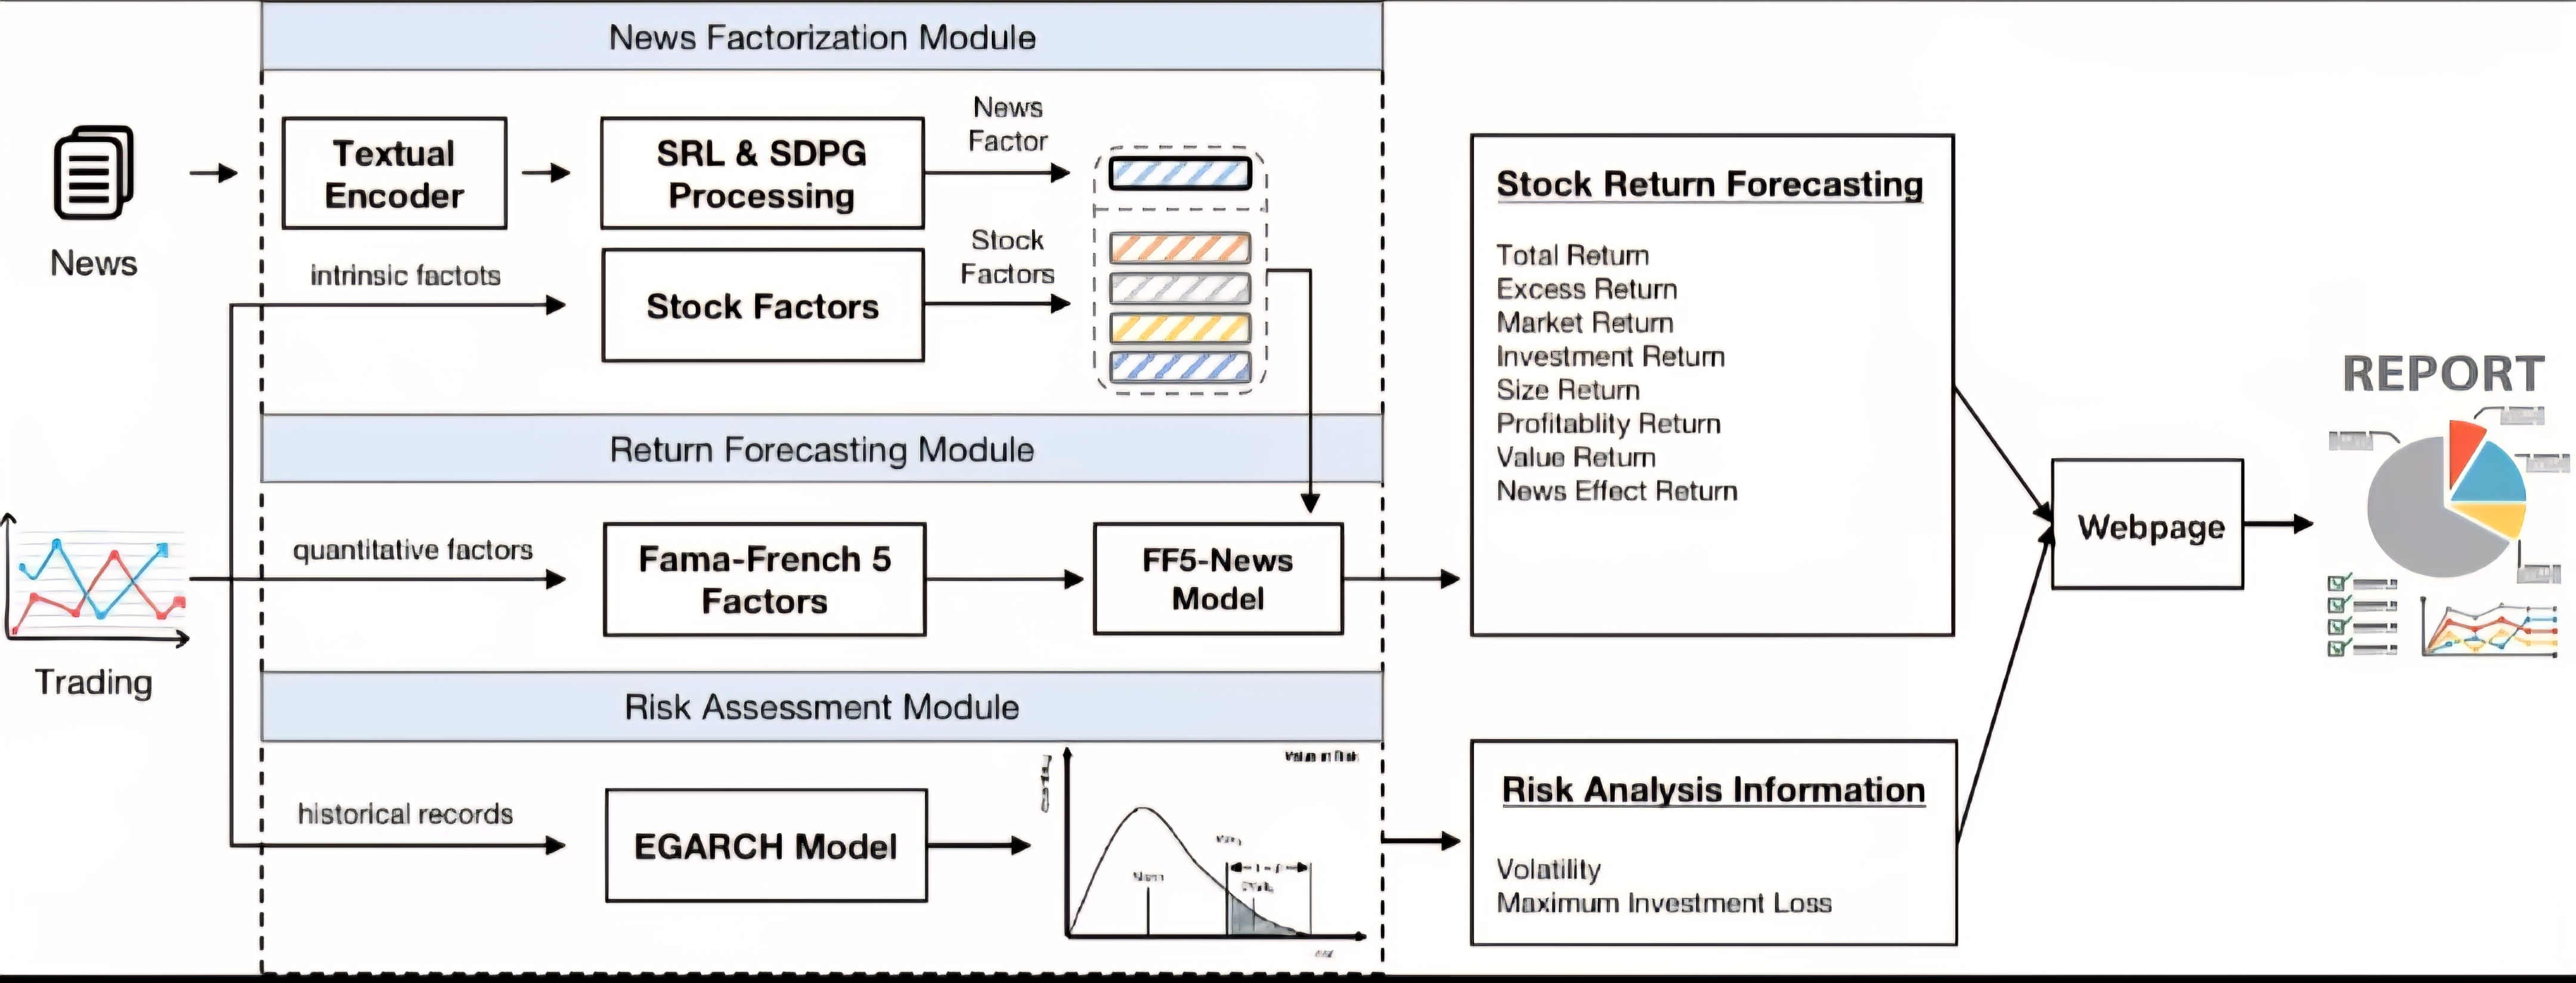
\includegraphics[width=0.90\textwidth]{flowchart.jpg} % Adjust width
    % 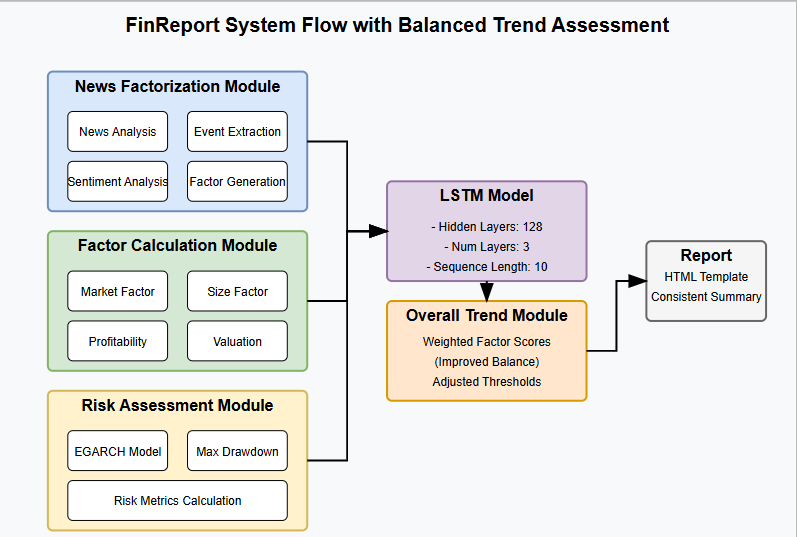
\includegraphics[height=3cm]{flowchart.png} % Adjust height
    % 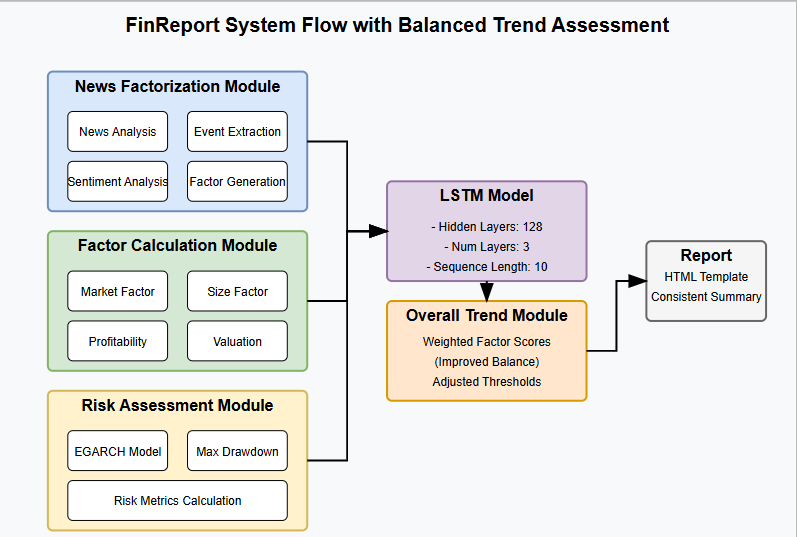
\includegraphics[scale=0.5]{flowchart.png} % Scale image
    % 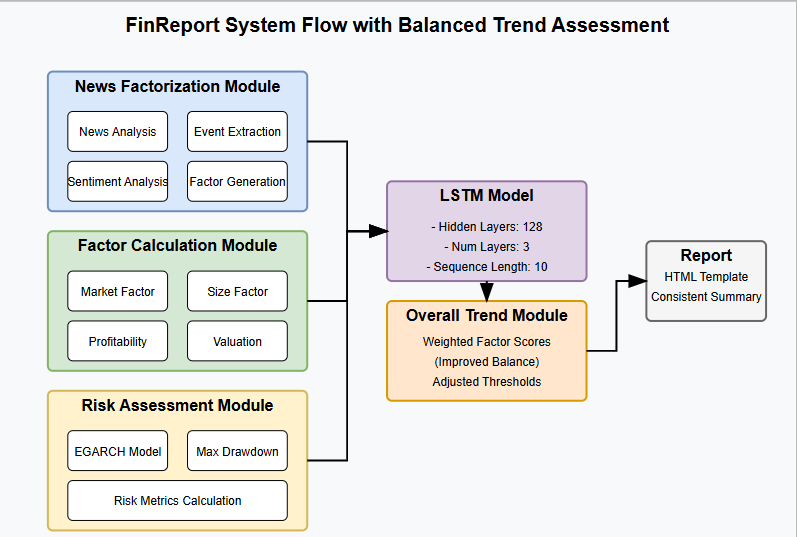
\includegraphics[width=0.5\textwidth, height=5cm, keepaspectratio]{flowchart.png} % Keep aspect ratio

    \caption{Proposed FinReport System Architecture}
    \label{fig:workflow_diagram}
\end{figure}
\subsection{{Data Integration Module}}
\begin{itemize}

\item \textbf{Historical Stock Data:} Time series data including price, volume, market value, and over 50 technical indicators (e.g., RSI, BIAS, MFI, CCI) from Chinese A-share stock databases spanning 2018-2021.
\item \textbf{Financial News:} Structured news items from financial news services, containing timestamps, headlines, and content text in both English and Chinese.
\item \textbf{Dataset Source:} We utilize the comprehensive Chinese stock market dataset \cite{FinReportDataset2025}, which contains historical stock data, financial news, and pre-computed technical indicators for Chinese A-share stocks spanning 2018-2021. This curated financial dataset includes 75 stocks from Shanghai and Shenzhen exchanges with 56 distinct feature columns including price data, trading metrics, technical indicators, and fundamental factors.
\item \textbf{Preprocessing Pipeline:} 

\begin{itemize}
\item \textbf{Missing Value Handling:} Forward-filling (LOCF - Last Observation Carried Forward) for technical indicators to maintain temporal continuity while preserving time series structure.
\item \textbf{Feature Normalization:} Z-score standardization of numerical features ($z = \frac{x - \mu}{\sigma}$) to facilitate neural network convergence.
\item \textbf{Outlier Treatment:} Winsorization at 1st and 99th percentiles to reduce impact of extreme values while preserving data distribution.
\item \textbf{Text Cleaning:} Removal of HTML artifacts, special characters, and duplicate information from news content using regex-based preprocessing.
\item \textbf{Technical Column Renaming:} Automatic detection and standardization of technical indicator column names for consistency across datasets.
\end{itemize}
\end{itemize}

As seen in our dataset \cite{FinReportDataset2025}, the integrated data combines structured numerical features (open, close, volume prices) with over 50 technical indicators and unstructured news text in the announcement column. This comprehensive integration creates a robust data foundation for multi-modal financial analysis.

\subsection{{News Factor Extraction Module}}
This module transforms unstructured financial news text into quantifiable sentiment and event metrics through a two-stage process:
\begin{itemize}
\item \textbf{Sentiment Analysis Pipeline:} 
\begin{itemize}
\item \textbf{FinBERT Implementation:} A domain-specific BERT model pre-trained on financial texts that produces raw sentiment scores in the range $[-1, +1]$, where -1 indicates highly negative sentiment and +1 indicates highly positive sentiment.
\item \textbf{Sentiment Augmentation:} Core sentiment scores are enhanced through financial keyword analysis (e.g., "profit", "loss", "revenue"), applying domain-specific weighting factors based on keyword importance.
\end{itemize}
\item \textbf{Event Extraction Engine:} 
\begin{itemize}
\item \textbf{Semantic Role Labeling (SRL):} The AllenNLP framework identifies grammatical relationships (subject-verb-object patterns) to capture structured financial events such as acquisitions, earnings announcements, and management changes.
\item \textbf{Financial Keyword Enhancement:} Domain-specific keyword dictionaries improve event recognition accuracy by incorporating finance-specific terminology.
\item Temporal Integration: Daily aggregation of multiple news items weighted by recency and relevance.
\end{itemize}
\vspace{0.10cm}
\item Module Interface with Forecasting Engine: 
\begin{itemize}
\item The sentiment scores are transmitted to the Market Factor and News Effect Factor computation functions.
\item Extracted events feed the Event Factor computation with structured \texttt{(event\_type, entities, magnitude)} tuples.
 \item Aggregated news sentiment over time generates a temporally aware sentiment curve for volatility estimation.
\end{itemize}
\item The dataset \cite{FinReportDataset2025} shows examples of complex news processing: the announcement column contains news about company performance updates, management changes, and market events. 
\end{itemize}
\subsection{{Return Forecasting Module}}
\subsubsection{{Market Factor}}
\begin{itemize}
    \item Inputs: \texttt{pct\_chg} (percentage change), volatility from \texttt{pct\_chg} series, sentiment from \texttt{news\_text}.
    \item Enhancement: Incorporates technical indicators (RSI, BIAS) for overbought/oversold conditions.
\end{itemize}

The market factor is computed using volatility-based impact with sentiment adjustment from the dataset \cite{FinReportDataset2025}:

\begin{equation}
\textbf{volatility} = \text{std}(\texttt{pct\_chg}_{recent\_5\_days}) \times 100
\end{equation}

\subsubsection{{Market Factor}}
\begin{itemize}
    \item \textbf{Inputs:} Daily percentage change (\texttt{pct\_chg}), news sentiment analysis from \texttt{news\_text}.
    \item \textbf{Purpose:} Captures market volatility effects and sentiment-driven momentum that influence individual stock returns.
\end{itemize}

The market factor implementation combines volatility analysis with news sentiment to determine market impact. The system computes recent volatility from the last 5 trading days and analyzes positive vs negative trading days:

\begin{equation}
\textbf{volatility} = \text{std}(\texttt{pct\_chg}_{\text{recent 5 days}}) \times 100
\end{equation}

Based on volatility levels, the factor applies different impact calculations:
- \textbf{High volatility} (> 4.0\%): Applies negative bias with volatility scaling
- \textbf{Moderate volatility} (> 2.5\%): Moderate negative impact with sentiment adjustment  
- \textbf{Low volatility}: Positive bias when more positive trading days exist, enhanced by news sentiment

The final factor value is amplified by 1.5x and includes random variation (±0.2) to reflect market uncertainty.

\subsubsection{{Size Factor}}
\begin{itemize}
    \item \textbf{Inputs:} Market capitalization data (\texttt{market\_value}), financial figures extracted from \texttt{news\_text}.
    \item \textbf{Purpose:} Captures size effects by analyzing market value changes and financial impact mentions in news.
\end{itemize}

The size factor evaluates market capitalization changes by comparing the latest market value to the historical average:

\begin{equation}
\textbf{diff\_ratio} = \frac{\texttt{market\_value}_{\text{latest}} - \texttt{market\_value}_{\text{average}}}{\texttt{market\_value}_{\text{average}}}
\end{equation}

The factor applies different scaling based on the magnitude of change:
- \textbf{Very large increase} (>25\%): Base effect 1.0 + scaled ratio
- \textbf{Significant increase} (10-25\%): Base effect 0.7 + scaled ratio  
- \textbf{Moderate changes} (-5\% to +5\%): Ratio scaled by factor of 3.0
- \textbf{Significant decreases}: Negative base effects with ratio scaling

The final factor incorporates news sentiment modifiers and financial impact mentions, then applies simple 2.5x base amplification with controlled randomization.

\begin{equation}
\textbf{size\_effect} = 
\begin{cases} 
1.0 + \min(\textbf{diff\_ratio} \times 0.1, 0.5), & \text{if diff\_ratio} > 0.25 \\
0.7 + \textbf{diff\_ratio} \times 0.5, & \text{if diff\_ratio} > 0.10 \\
0.5 + \textbf{diff\_ratio} \times 0.5, & \text{if diff\_ratio} > 0.05 \\
\textbf{diff\_ratio} \times 3.0, & \text{if } -0.05 < \textbf{diff\_ratio} \leq 0.05 \\
-0.5 + \textbf{diff\_ratio} \times 2.0, & \text{if diff\_ratio} > -0.10 \\
-1.0 + \max(\textbf{diff\_ratio} \times 0.1, -0.5), & \text{otherwise}
\end{cases}
\end{equation}

\begin{equation}
\textbf{Range: } -1.5 \leq \textbf{size\_effect} \leq +1.5
\end{equation}

Additional adjustments are made based on financial figures extracted from \texttt{news\_text} (yi yuan, wan yuan mentions).

\subsubsection{{Valuation Factor}}
\begin{itemize}
    \item \textbf{Inputs:} Valuation metrics from dataset columns \cite{FinReportDataset2025} (Book-to-Market, Dividend Yield, Sales-to-Price ratio, etc.), profit/loss terms from \texttt{news\_text}.
    \item \textbf{Purpose:} Evaluates investment value by analyzing available valuation metrics and sector-specific news sentiment.
\end{itemize}

The valuation factor checks for multiple valuation-related columns in the dataset \cite{FinReportDataset2025}:

\begin{itemize}
    \item \texttt{value\_factor\_Book\_to\_Market\_Equity}
    \item \texttt{value\_factor\_Dividend\_Yield}  
    \item \texttt{value\_factor\_Sales\_to\_Price\_Ratio}
    \item \texttt{value\_factor\_Assets\_to\_Market\_Equity}
\end{itemize}

When valuation data is available, the factor calculates percentage changes from historical values. When unavailable, it relies on sector-specific sentiment analysis with different impact weights:

\textbf{Sector-Specific Adjustments:}
\begin{itemize}
    \item \textbf{Technology:} $+0.3$ (positive sentiment) / $-0.2$ (negative sentiment)
    \item \textbf{Pharmaceutical:} $+0.2$ (positive sentiment) / $-0.3$ (negative sentiment)
    \item \textbf{Financial:} $+0.2$ (positive sentiment) / $-0.3$ (negative sentiment)
    \item \textbf{Energy:} $+0.15$ (positive sentiment) / $-0.25$ (negative sentiment)
\end{itemize}

The factor also incorporates profit/loss keyword analysis and percentage change extraction from news text, using consistent base amplification.

\begin{equation}
\textbf{valuation\_effect} = 
\begin{cases} 
\textbf{diff\_ratio} \times 0.25, & \text{if valuation columns available} \\
\textbf{sector\_adjustment} \times \textbf{sentiment}, & \text{based on news analysis}
\end{cases}
\end{equation}

\begin{equation}
\textbf{Range: } -1.0 \leq \textbf{value} \leq +1.0
\end{equation}

Where sector adjustments range from 0.1 to 0.3 for positive sentiment and -0.15 to -0.3 for negative sentiment.

\subsubsection{{Profitability Factor}}
\begin{itemize}
    \item \textbf{Inputs:} Profitability metrics from dataset \cite{FinReportDataset2025} (EPS, net profit margin, ROE, ROA, gross/net profit), profit-related keywords from \texttt{news\_text}.
    \item \textbf{Purpose:} Evaluates corporate profitability through quantitative metrics when available, or sentiment analysis of earnings-related news content.
\end{itemize}

The profitability factor first searches for available profitability columns in the dataset:
- \texttt{eps}, \texttt{net\_profit\_margin}, \texttt{roe}, \texttt{roa}, \texttt{grossprofit}, \texttt{netprofit}

When profitability data exists, it calculates percentage change between current and previous values, scaled by factor 0.05 and capped at ±1.5.

When quantitative data is unavailable, the factor analyzes news content for:
- \textbf{Earnings keywords:} profit, earnings, income, revenue, margin, EPS, ROE, ROI
- \textbf{Directional terms:} increase/decrease, rise/fall, improve/decline
- \textbf{Percentage changes:} Extracted numeric percentages from text

The factor applies strong negative bias (-1.8) for explicit loss mentions but scales positive profit increases with sentiment modifiers, using standard base amplification.

\begin{equation}
\textbf{Range: } -3.0 \leq \textbf{profitability\_effect} \leq +3.0
\end{equation}


\vspace{0.20 cm}
\subsubsection{{Investment Factor}}
\begin{itemize}
    \item \textbf{Inputs:} Investment-related financial figures extracted from \texttt{news\_text}, acquisition/expansion keywords, R\&D mentions.
    \item \textbf{Purpose:} Quantifies corporate investment activity impact by analyzing investment amounts and strategic activity mentions in news.
\end{itemize}

The investment factor analyzes news content for investment-related information:
- \textbf{Investment amounts:} Extracts numeric financial figures from news text
- \textbf{Activity types:} Counts mentions of acquisition, expansion, R\&D activities
- \textbf{Sentiment context:} Applies positive/negative weighting to investment news

The factor calculates base effects from investment amounts when available, or relies on sentiment analysis when amounts are not specified. Activity type multipliers are applied:
- Acquisition activities: +0.6 per mention
- Expansion activities: +0.5 per mention  
- R\&D activities: +0.7 per mention

Final values are capped in the range [0.0, +2.0] as investment activities are typically viewed positively for long-term growth prospects.

\begin{equation}
\textbf{investment\_effect} = \textbf{impact\_scale} \times 0.5 \times 
\begin{cases} 
1.0, & \text{if } \textbf{news\_sentiment} > 0 \\
0.5, & \text{otherwise}
\end{cases}
\end{equation}

\begin{equation}
\textbf{Range: } -1.0 \leq \textbf{investment\_effect} \leq +1.5
\end{equation}

\subsubsection{{News Effect Factor}}
\begin{itemize}
    \item \textbf{Input:} Sentiment analysis of \texttt{news\_text} using TextBlob and keyword-based analysis with financial terms.
    \item \textbf{Purpose:} Converts unstructured news content into quantified sentiment scores that directly influence return predictions.
\end{itemize}

The news effect factor combines two sentiment analysis approaches:

\textbf{1. Keyword Analysis:} Counts positive and negative financial keywords from predefined dictionaries:
- \textbf{Positive:} increase, rise, grow, profit, improved, partnership, acquisition, dividend, earnings, success
- \textbf{Negative:} decrease, decline, loss, warning, investigation, lawsuit, delay, weak, miss, reduced

\textbf{2. TextBlob Sentiment:} Applies natural language processing for polarity analysis of the complete news text.

The final sentiment combines both approaches:
\begin{equation}
\textbf{combined\_sentiment} = \frac{\textbf{TextBlob\_polarity} + \textbf{keyword\_sentiment}}{2}
\end{equation}

The news factor applies different scaling based on sentiment strength:
- Very positive ($\geq 0.5$): Random range [0.7, 1.2] 
- Moderately positive (>0): Random range [0.3, 0.7]
- Moderately negative (>-0.5): Random range [-0.7, -0.3]  
- Very negative ($\leq -0.5$): Random range [-1.2, -0.7]

Final amplification of 2.0x is applied, with range [-2.0, +2.0].

Where keywords are extracted from the dataset's parsed Chinese text including:
\begin{itemize}
    \item Positive: [zengzhang, yingli, shangsheng, huode, chenggong, tisheng, shouyi] (growth, profit, rise, gain, success, improvement, revenue)
    \item Negative: [xiajiang, kuisun, jianshao, jinggao, zhaiwu, diaocha, weigui] (decline, loss, decrease, warning, debt, investigation, violation)
\end{itemize}

\begin{equation}
\textbf{combined\_sentiment} = \frac{\textbf{base\_sentiment} + \textbf{keyword\_sentiment}}{2}
\end{equation}

\begin{equation}
\textbf{news\_effect} = \textbf{combined\_sentiment} \times 2.0 \text{ (amplification)}
\end{equation}

\begin{equation}
\textbf{Range: } -2.0 \leq \textbf{news\_effect} \leq +2.0
\end{equation}


These factors are formatted through our custom display formatting system, which rounds values to one decimal place and creates clear descriptions for interpretability. The factor calculations reference the Chinese stock market dataset structure \cite{FinReportDataset2025}, which contains historical stock data, financial news, and pre-computed technical indicators for Chinese A-share stocks spanning 2018-2021, with the main dataset providing structured access to 56 feature columns across 75 stocks.

All factors undergo enhancement using the amplification process detailed in Section 3.5.1 before being combined for overall trend calculation.

\subsection{{Risk Assessment Module}}
\begin{itemize}
    \item \textbf{Purpose:} Quantifies investment risk through multiple complementary metrics including volatility clustering, tail risk, and sequential loss patterns.
    \item \textbf{Implementation:} Uses advanced econometric models (EGARCH) combined with historical simulation methods.
\end{itemize}

This module provides comprehensive risk assessment through five integrated components:

\subsubsection{{EGARCH-Based Volatility Modeling}}
The Exponential Generalized Autoregressive Conditional Heteroskedasticity (EGARCH) model captures asymmetric volatility responses where negative market shocks impact future volatility more than positive shocks:

\begin{equation}
\ln(\sigma_t^2) = \omega + \beta \ln(\sigma_{t-1}^2) + \alpha \frac{|r_{t-1}|}{\sigma_{t-1}} + \gamma \frac{r_{t-1}}{\sigma_{t-1}}
\end{equation}

\textbf{Parameter Interpretation:}
\begin{itemize}
    \item $\omega$: Long-term volatility baseline
    \item $\beta$: Volatility persistence (typically 0.85-0.95)
    \item $\alpha$: Magnitude effect of past shocks
    \item $\gamma$: Asymmetry parameter (negative for leverage effect)
\end{itemize}

\textbf{95\% Value at Risk (VaR) Computation:}
\begin{equation}
\text{VaR}_{95} = 1.65 \times \sigma_t
\end{equation}

\begin{equation}
\text{volatility\_score} = \min(\sigma_t \times 100, 10.0) \quad \text{(capped at 10)}
\end{equation}

The EGARCH model is implemented using the \texttt{arch} Python package, providing robust parameter estimation through maximum likelihood methods.
\subsubsection{{Maximum Drawdown Analysis}}
Maximum Drawdown (MDD) quantifies the largest peak-to-trough decline, capturing sequential loss patterns invisible to point-in-time volatility measures:

\begin{equation}
\text{MDD}_t = \max_{0 \leq s \leq t} \left[ \frac{P_s - P_t}{P_s} \right]
\end{equation}

where $P_t$ represents the portfolio value at time $t$. The drawdown score is computed as:

\begin{equation}
\text{drawdown\_score} = \min(|\text{MDD}| \times 10, 10.0)
\end{equation}

\subsubsection{{Return-Based Risk Assessment}}
The return score inversely relates to expected performance, penalizing both very high and very low predicted returns:

\begin{equation}
\text{return\_score} = 5 - \min(\max(\text{predicted\_return} \times 2, -5), 5)
\end{equation}

\subsubsection{{Conditional Value at Risk (CVaR)}}
CVaR provides tail risk assessment by averaging losses exceeding the VaR threshold:

\begin{equation}
\text{CVaR}_{95} = E[R | R \leq -\text{VaR}_{95}]
\end{equation}

Implementation uses historical simulation over a 252-day rolling window, providing more coherent risk measurement than standard VaR in extreme market conditions.

\subsubsection{{Weighted Risk Score Integration}}
The final risk assessment combines all components through empirically-determined weights:

\begin{equation}
\text{weighted\_risk\_score} = 0.5 \times \text{volatility\_score} + 0.3 \times \text{drawdown\_score} + 0.2 \times \text{return\_score}
\end{equation}

\textbf{Risk Classification Thresholds:}
\begin{itemize}
    \item \textbf{Substantial Risk:} $> 7.5$ (Extreme market stress conditions)
    \item \textbf{High Risk:} $> 6.0$ (Above-average volatility with significant drawdown potential)
    \item \textbf{Moderate-High:} $> 4.5$ (Elevated risk requiring careful monitoring)
    \item \textbf{Moderate:} $> 3.0$ (Standard market risk levels)
    \item \textbf{Low-Moderate:} $> 1.5$ (Below-average risk environment)
    \item \textbf{Favorable:} $\leq 1.5$ (Low-risk, stable market conditions)
\end{itemize} 
The dataset's \cite{FinReportDataset2025} \textbf{volatility\_factor\_Total\_Volatility} and related columns provide direct inputs for risk calculations, while temporal price data (\texttt{open}, \texttt{close}, \texttt{high}, \texttt{low}) enables return computation for maximum drawdown and CVaR estimation.

\subsection{{Factor Enhancement and Overall Trend Calculation}}
\begin{itemize}
    \item \textbf{Purpose:} Combines individual factor signals into a unified directional forecast while preserving interpretability through consistent amplification.
    \item \textbf{Approach:} Multi-stage amplification followed by weighted aggregation using the enhancement mechanism described in Section 3.2.6.
\end{itemize}

\subsubsection{{Factor Weight Specification}}
Individual factors are combined using empirically-determined weights based on their predictive power and stability:

\begin{equation}
\textbf{W} = 
\begin{bmatrix} 
\text{market\_factor} & 0.15 \\ 
\text{size\_factor} & 0.15 \\ 
\text{valuation\_factor} & 0.10 \\ 
\text{profitability\_factor} & 0.15 \\ 
\text{investment\_factor} & 0.20 \\ 
\text{news\_effect\_factor} & 0.10 \\ 
\text{event\_factor} & 0.25
\end{bmatrix}
\end{equation}

The event factor receives the highest weight (0.25) due to its strong predictive power for short-term price movements and immediate market reactions, followed by the investment factor (0.20) for medium-term price movements, while valuation and news factors receive lower weights (0.10) reflecting their longer-term impact horizons.

\subsubsection{{Factor Enhancement Process}}
Before computing the weighted sum, factors undergo the amplification enhancement process described in Section 3.2.6 to ensure adequate signal strength:

\textbf{Base Amplification:}
All factor values are enhanced using a fixed 2.5x multiplier to ensure meaningful signal strength:
\begin{equation}
\textbf{enhanced\_factor}_i = \textbf{factor}_i \times 2.5
\end{equation}

\textbf{Trend-Based Enhancement:}
When factors align with the overall market direction (determined by counting positive vs. negative factor values), additional amplification is applied:
\begin{equation}
\textbf{trend\_multiplier} = 
\begin{cases} 
1.3, & \text{if factor direction matches dominant trend} \\
1.0, & \text{otherwise}
\end{cases}
\end{equation}

\textbf{Final Processing:}
Randomization (0.9 to 1.1 multiplier) and value capping ensure realistic bounds while preserving directional signals:
\begin{equation}
\tilde{f}_i = \text{clamp}\left(\textbf{enhanced\_factor}_i \times \textbf{trend\_multiplier} \times \text{random}(0.9, 1.1), -5.0, 5.0\right)
\end{equation}

\subsubsection{{Weighted Aggregation}}
The final trend score combines all enhanced factors using the original factor weights:

\begin{equation}
\text{Trend\_Score} = \sum_{i=1}^{7} \left(\tilde{f}_i \times w_i\right) + 0.15
\end{equation}

where the positive bias (+0.15) reflects long-term upward equity market drift observed in historical data, and $w_i$ are the original factor weights defined above.

\subsubsection{{Qualitative Classification}}
The trend score is mapped to interpretable categories using empirically-calibrated thresholds:

\begin{equation}
\text{Classification} = 
\begin{cases} 
\textbf{Strongly Positive}, & \text{if Score} > +1.2 \\
\textbf{Positive}, & \text{if } +0.4 < \text{Score} \leq +1.2 \\
\textbf{Neutral}, & \text{if } -0.4 \leq \text{Score} \leq +0.4 \\
\textbf{Negative}, & \text{if } -1.2 \leq \text{Score} < -0.4 \\
\textbf{Strongly Negative}, & \text{if Score} < -1.2
\end{cases}
\end{equation}

\subsection{Dynamic Report Generation Module}
The FinReport system generates HTML-based reports designed specifically for maximum interpretability:
\begin{itemize}
    \item Visual Hierarchy: The report structure follows a top-down information hierarchy, placing the most critical insights (overall trend and summary) at the top, followed by factor-specific details and risk metrics.
\item Color-Coding Philosophy: Positive impacts use the CSS class 'positive' (red) and negative impacts use 'negative' (green), deliberately inverting Western color conventions to align with Chinese market cultural context where red represents prosperity and upward movement.
\item Numerical Precision Control: All percentage values are consistently rounded to one decimal place to maintain visual uniformity and prevent false precision from influencing decision-making.
\item Explanatory Language Templates: The system employs a diverse set of pre-configured language templates for each factor and risk level, selected based on factor magnitude and direction to provide natural language explanations that convey both the quantitative impact and qualitative significance.
\item Consistency Enforcement: The report generation module includes consistency checks to ensure that factor descriptions align with the overall trend assessment, preventing contradictory messaging that could confuse interpretation.
\item This carefully designed reporting approach ensures that complex quantitative analyses are translated into actionable insights accessible to both technical and non-technical stakeholders, while maintaining the transparency necessary for informed investment decisions.
\end{itemize}

\vspace{0.20cm}
\section{Algorithm}

\subsection{Return Forecast Calculation}

The return forecast is computed using a weighted \allowbreak combination of multiple factors, where the \textbf{event factor receives the highest weight (0.25)} due to its immediate impact on market sentiment and price movements.
\begin{align}
\mathbf{predicted\_return} &= 0.10 \times \mathbf{market\_factor} + 0.15 \times \mathbf{size\_factor} + 0.10 \times \mathbf{valuation\_factor} \nonumber \\
&\quad + 0.10 \times \mathbf{profitability\_factor} + 0.20 \times \mathbf{investment\_factor} \nonumber \\
&\quad + 0.10 \times \mathbf{news\_effect\_factor} + \mathbf{0.25} \times \mathbf{event\_factor} + 0.15
\end{align}


Each factor is calculated as follows:

\vspace{0.10cm}
\text{I) Market Factor}
\begin{enumerate}
    \item \text{Extract Recent Volatility:}
    \begin{itemize}
        \item Compute standard deviation of \texttt{pct\_chg} over the last 5 days.
        \item Multiply by 100 to get volatility.
    \end{itemize}
    \vspace{0.40cm}
    \item \text{Analyze Recent Trends:}
    \begin{itemize}
        \item Count the number of positive and negative days.
    \end{itemize}

    \item \text{Perform Sentiment Analysis:}
    \begin{itemize}
        \item Compute sentiment score from \texttt{news\_text}.
    \end{itemize}

    \item \text{Determine Base Impact:}
    \begin{itemize}
        \item If volatility $> 4.0$, assign a strong negative impact.
        \item If $2.5 < \text{volatility} \leq 4.0$, assign moderate negative impact.
        \item If positive days $>$ negative days, adjust positively using sentiment.
        \item Otherwise, adjust slightly negatively.
    \end{itemize}

    \item \text{Enhance with Technical Indicators (RSI):}
    \begin{itemize}
        \item If RSI $> 70$, reduce impact (overbought condition).
        \item If RSI $< 30$, increase impact (oversold condition).
    \end{itemize}

    \item \text{Return Final Market Factor:}
    \begin{itemize}
        \item Multiply final impact by $1.5$ for amplification.
    \end{itemize}
\end{enumerate}
\text{II) Size Factor}
\begin{enumerate}
    \item \text{Compute Size Change Percentage:}
    \begin{itemize}
        \item Extract the latest market value.
        \item Compute the average market value.
        \item Calculate the percentage difference:
       \begin{equation}
\bm{\textbf{diff\_ratio} = \frac{\textbf{latest\_val} - \textbf{avg\_val}}{\textbf{avg\_val}}}
\end{equation}

    \end{itemize}

    \item \text{Extract Financial Impact from News:}
    \begin{itemize}
        \item Analyze \texttt{news\_text} for financial figures.
    \end{itemize}

\item \text{Determine Base Effect Based on Market Value Change:}
    \begin{itemize}
        \item If $\text{diff\_ratio} > 0.25$, apply strong positive impact.
        \item If $0.10 < \text{diff\_ratio} \leq 0.25$, apply moderate positive impact.
        \item If $0.05 < \text{diff\_ratio} \leq 0.10$, apply slight positive impact.
        \item If $-0.05 \leq \text{diff\_ratio} \leq 0.05$, apply neutral impact with minor variations.
        \item If $-0.10 < \text{diff\_ratio} \leq -0.05$, apply slight negative impact.
        \item If $-0.25 < \text{diff\_ratio} \leq -0.10$, apply moderate negative impact.
        \item If $\text{diff\_ratio} \leq -0.25$, apply strong negative impact.
    \end{itemize}

    \item \text{Return Final Size Factor}
    \begin{itemize}
        \item Multiply the computed effect by $1.5$ for amplification.
    \end{itemize}
\end{enumerate}
\text{III) Profitability Factor}
\begin{enumerate}
    \item \text{Identify Profitability Metrics:}
    \begin{itemize}
        \item Define key financial metrics: 
        \{EPS, Net Profit Margin, ROE, ROA, Gross Profit, Net Profit\}.
        \item Identify available metrics in the dataset.
    \end{itemize}

    \item \text{Extract Profit-Related Information from News:}
    \begin{itemize}
        \item Extract \text{profit increases} from \texttt{news\_text}.
        \item Extract \text{profit decreases} from \texttt{news\_text}.
    \end{itemize}


    \item \text{Determine Base Effect:}
    \begin{itemize}
        \item If at least \text{one profitability metric} is available:
        \begin{itemize}
            \item Compute percentage change between the most recent and previous values.
            \item Scale down the impact.
        \end{itemize}
        \item If \texttt{news\_text} contains \text{"net loss"} or \text{"loss"}, set a strong negative effect.
        \item If \text{profit increases} are found, apply a positive adjustment.
        \item If \text{profit decreases} are found, apply a negative adjustment.
        \item Otherwise, adjust based on sentiment analysis.
    \end{itemize}

    \item \text{Return Final Profitability Factor:}
    \begin{itemize}
        \item Multiply the computed effect by $1.5$ for amplification.
    \end{itemize}
\end{enumerate}
\text{IV) Valuation Factor}
\begin{enumerate}
    \item \text{Identify Valuation Metrics:}
    \begin{itemize}
        \item Define key valuation metrics: 
        \{Book-to-Market Equity, Dividend Yield, Sales-to-Price Ratio\}.
        \item Identify available metrics in the dataset.
    \end{itemize}

    \item \text{Analyze News Sentiment and Sector:}
    \begin{itemize}
        \item Perform \text{sentiment analysis} on \texttt{news\_text}.
        \item Identify the \text{sector} associated with the company.
    \end{itemize}

    \item \text{Determine Base Effect:}
    \begin{itemize}
        \item If at least one \text{valuation metric} is available:
        \begin{itemize}
            \item Compute the \text{difference ratio} between the latest value and its benchmark.
            \item Scale the impact using a factor of $0.25$.
        \end{itemize}
        \item Otherwise, apply \text{sector-specific adjustments}:
        \begin{itemize}
            \item \text{Pharmaceuticals:} $+0.2$ (positive sentiment), $-0.3$ (negative sentiment).
            \item \text{Technology:} $+0.3$ (positive sentiment), $-0.2$ (negative sentiment).
            \item \text{General market:} $+0.15$ (positive sentiment), $-0.2$ (negative sentiment).
            \item \text{Default adjustment:} $+0.1$ (positive sentiment), $-0.1$ (negative sentiment).
        \end{itemize}
    \end{itemize}

    \item \text{Return Final Valuation Factor.}
\end{enumerate}
\text{V) Investment Factor}
\begin{enumerate}
    \item \text{Extract Investment Amount from News:}
    \begin{itemize}
        \item Identify mentions of investments in \text{billion yuan} using a regex pattern.
        \item Convert extracted values to numerical amounts.
    \end{itemize}

    \item \text{Analyze Investment Types in News:}
    \begin{itemize}
        \item Count occurrences of acquisitions and mergers (M\&A).
        \item Count mentions of \text{business expansion} (new facilities, capacity increase).
        \item Count references to research and development (R\&D) activities.
    \end{itemize}

    \item \text{Determine Base Effect:}
    \begin{itemize}
        \item If investment amounts are found:
        \begin{itemize}
            \item Assign a \text{base effect} based on investment size:
            \begin{itemize}
                \item $> 50$ billion yuan $\rightarrow 2.5$
                \item $> 20$ billion yuan $\rightarrow 2.0$
                \item $> 10$ billion yuan $\rightarrow 1.5$
                \item $> 5$ billion yuan $\rightarrow 1.0$
                \item $> 1$ billion yuan $\rightarrow 0.7$
                \item Otherwise $\rightarrow 0.4$
            \end{itemize}
        \end{itemize}
        \item If no investment amount is found:
        \begin{itemize}
            \item Adjust based on \text{sentiment analysis}: $+0.5$ for positive, $-0.5$ for negative.
        \end{itemize}
    \end{itemize}

    \item \text{Modify Effect Based on Investment Types:}
    \begin{itemize}
        \item Acquisitions $\rightarrow +0.6$ per mention.
        \item Expansions $\rightarrow +0.5$ per mention.
        \item R\&D mentions $\rightarrow +0.7$ per mention.
    \end{itemize}

    \item \text{Return Final Investment Factor.}

\end{enumerate}
\text{VI) News Effect Factor}
\begin{enumerate}
    \item \text{Determine Base Effect from Sentiment Score:}
    \begin{itemize}
    \item If \textit{sentiment score} $\geq 0.5$ $\rightarrow$ assign a random positive effect between $0.7$ and $1.2$.
    \item If $0 <$ \textit{sentiment score} $< 0.5$ $\rightarrow$ assign a random positive effect between $0.3$ and $0.7$.
    \item If $-0.5 <$ \textit{sentiment score} $\leq 0$ $\rightarrow$ assign a random negative effect between $-0.7$ and $-0.3$.
    \item If \textit{sentiment score} $\leq -0.5$ $\rightarrow$ assign a random negative effect between $-1.2$ and $-0.7$.
\end{itemize}


    \item \text{Analyze Specific News Content:}
    \begin{itemize}
        \item Check for keywords related to \text{earnings \& financials} (e.g., ``profit'', ``revenue'').
        \item Check for mentions of \text{forecast \& guidance} (e.g., ``outlook'', ``expectations'').
        \item Detect \text{management changes} (e.g., ``CEO'', ``executive'').
        \item Identify \text{regulatory/legal issues} (e.g., ``compliance'', ``litigation'').
    \end{itemize}

    \item \text{Adjust Base Effect Based on Content:}
    \begin{itemize}
        \item \text{Earnings-related news:} 
        \begin{itemize}
            \item Add $+0.3$ if sentiment is positive.
            \item Subtract $-0.3$ if sentiment is negative.
        \end{itemize}
        \item \text{Guidance-related news:}
        \begin{itemize}
            \item Add $+0.2$ if sentiment is positive.
            \item Subtract $-0.2$ if sentiment is negative.
        \end{itemize}
        \item \text{Management changes:}
        \begin{itemize}
            \item Add $+0.2$ if sentiment is positive.
            \item Subtract $-0.2$ if sentiment is negative.
        \end{itemize}
        \item \text{Regulatory news:}
        \begin{itemize}
            \item Always subtract $-0.3$, as it is usually negative.
        \end{itemize}
    \end{itemize}

    \item \text{Apply Final Amplification Factor:}
    \begin{itemize}
        \item Multiply the computed effect by $2.0$ to enhance the impact.
    \end{itemize}
\end{enumerate}
\text{VII) Event Factor}
\begin{enumerate}
    \item \text{Define Event Keywords:}
    \begin{itemize}
        \item Create a list of \text{positive market events} (e.g., ``acquisition'', ``partnership'', ``approval'').
        \item Create a list of \text{negative market events} (e.g., \allowbreak``lawsuit'', ``litigation'', ``investigation'').
    \end{itemize}

    \item \text{Count Event Occurrences:}
    \begin{itemize}
        \item Convert \texttt{news\_text} to \text{lowercase} for case-insensitive comparison.
        \item Count how many \text{positive events} appear in the text.
        \item Count how many \text{negative events} appear in the text.
    \end{itemize}

    \item \text{Extract Financial Impact (if any):}
    \begin{itemize}
        \item Use \textit{extract\_financial\_figures(news\_text)} to determine any financial impact.
    \end{itemize}

    \item \text{Compute Base Effect:}
    \begin{itemize}
        \item If \text{positive event count $>$ negative event count}, assign a \text{positive effect} (capped at $2.0$).
        \item If \text{negative event count $>$ positive event count}, assign a \text{negative effect} (capped at $-2.0$).
        \item If counts are \text{equal}, set base effect to \text{0.0}.
    \end{itemize}

    \item \text{Adjust Based on Financial Impact:}
    \begin{itemize}
        \item Scale financial impact (max value $1.0$).
        \item If base effect is \text{positive}, increase it by the scaled financial impact.
        \item If base effect is \text{negative}, increase it by \text{half} of the scaled financial impact (to reduce negativity).
    \end{itemize}

\end{enumerate}
All factors are enhanced using a straightforward amplification algorithm that increases each factor's impact while maintaining directional consistency:

\text{VIII) Factor Amplification}
\begin{enumerate}
    \item \text{Extract Factor Values:}
    \begin{itemize}
        \item Retrieve values from each input factor dictionary.
        \item Use \texttt{get('value', 0.0)} to ensure safe access.
    \end{itemize}

    \item \text{Define Base Amplification:}
    \begin{itemize}
        \item Set base multiplier: $2.5$.
    \end{itemize}

    \item \text{Count Dominant Factors:}
    \begin{itemize}
        \item Count \text{positive factors} (values $> 0.5$).
        \item Count \text{negative factors} (values $< -0.5$).
    \end{itemize}

    \item \text{Determine Market Trend:}
    \begin{itemize}
        \item If $\text{positive count} \geq 3$ and exceeds negative count $\Rightarrow$ \text{Upward trend}.
        \item If $\text{negative count} \geq 3$ and exceeds positive count $\Rightarrow$ \text{Downward trend}.
        \item Otherwise, trend is \text{Mixed}.
    \end{itemize}

    \item \text{Apply Simple Enhancement:}
    \begin{itemize}
        \item Apply trend multiplier: $1.3$ if factor aligns with dominant trend.
        \item Add randomization: multiply by random value between $0.9$ and $1.1$.
        \item Compute enhanced value: 
        \begin{equation}
\bm{\textbf{enhanced\_value} = \textbf{original\_value} \times 2.5 \times \textbf{trend\_multiplier} \times \textbf{random\_factor}}
\end{equation}

        \item Cap final values between $[-5.0, 5.0]$ to ensure reasonable bounds.
    \end{itemize}

    \item \text{Return Enhanced Factors:}
    \begin{itemize}
        \item Store all updated values in a structured dictionary.
    \end{itemize}

\end{enumerate}
\subsection{Risk Assessment Methodology}
The risk assessment uses a sophisticated approach combining multiple risk metrics.
\begin{enumerate}
    \item \text{Extract Risk Metrics:}
    \begin{itemize}
        \item Volatility, Max Drawdown, VaR (95\%), Conditional VaR, Risk-Adjusted Ratio.
    \end{itemize}

    \item \text{Classify Volatility:}
    \begin{itemize}
        \item Extreme: $volatility > 0.15$  $\Rightarrow$ Cap decline at $25\%$.
        \item High: $volatility > 0.10$  $\Rightarrow$ Cap decline at $20\%$.
        \item Elevated: $volatility > 0.07$.
        \item Moderate: $volatility > 0.04$.
        \item Low: $volatility \leq 0.04$ $\Rightarrow$ At least $2\%$.
    \end{itemize}

    \item \text{Compute Weighted Risk Score:}
\begin{align}
\textbf{risk\_score} =\ & (0.4 \times \textbf{vol\_score}) + (0.25 \times \textbf{drawdown\_score}) \nonumber \\
& + (0.15 \times \textbf{var\_score}) + (0.2 \times \textbf{return\_risk})
\end{align}

    \item \text{Assign Risk Level Based on Score:}
    \begin{itemize}
        \item Substantial risk: $risk\_score > 7.5$.
        \item High risk: $risk\_score > 6.0$.
        \item Moderate-High risk: $risk\_score > 4.5$.
        \item Moderate risk: $risk\_score > 3.0$.
        \item Low-Moderate risk: $risk\_score > 1.5$.
        \item Favorable risk: $risk\_score \leq 1.5$.
    \end{itemize}

    \item \text{Generate Risk Assessment Summary:}
    \begin{itemize}
        \item Output: Maximum expected decline, Volatility class, Risk level.
    \end{itemize}

\end{enumerate}
\vspace{1.5cm}
Individual risk metrics are calculated as follows:
\vspace{0.10cm}

\text{1) Volatility (EGARCH-based):}
\begin{equation}
\bm{\ln(\sigma_t^2) = \omega + \beta \ln(\sigma_{t-1}^2) + \alpha \frac{|r_{t-1}|}{\sigma_{t-1}} + \gamma \frac{r_{t-1}}{\sigma_{t-1}}}
\end{equation}
where:
\begin{itemize}
    \item $\sigma_t^2$ is the conditional variance at time $t$.
    \item $\omega, \beta, \alpha, \gamma$ are model parameters.
    \item $\bm{r_{t-1}}$ is the previous return.
\end{itemize}

\begin{center}
95\% Value at Risk (VaR)
\end{center}

\text{2) Maximum Drawdown:}
\begin{algorithm}
\caption{Maximum Drawdown}
\label{alg:max_drawdown}
\begin{algorithmic}[1]
    \Require Returns series \( R \) of length \( n \)
    \Ensure Maximum Drawdown (MDD)
    
    \State Initialize \( C \gets 1 \) \Comment{Cumulative return starts at 1}
    \State Initialize \( M \gets 1 \) \Comment{Running maximum return}
    \State Initialize \( D \gets 0 \) \Comment{Maximum drawdown}

    \For{\( t = 1 \) to \( n \)}
        \State \( C \gets C \times (1 + R_t) \) \Comment{Update cumulative return}
        \State \( M \gets \max(M, C) \) \Comment{Update running maximum}
        \State \( D_t \gets \frac{C - M}{M} \) \Comment{Compute drawdown}
        \State \( D \gets \min(D, D_t) \) \Comment{Update maximum drawdown}
    \EndFor

    \State \Return \( D \)
\end{algorithmic}
\end{algorithm}

\vspace{1cm}

\text{3) Condition Value at Risk:}
\begin{algorithm}
\caption{Conditional Value at Risk (CVaR)}
\label{alg:cvar}
\begin{algorithmic}[1]
    \Require Returns series $R$ of length $n$, confidence level $\alpha$
    \Ensure Conditional Value at Risk (CVaR)
    \State \textbf{Sort} $R$ in ascending order 
    \State \textbf{Compute} Value at Risk (VaR): $V \gets$ percentile of $R$ at $100\alpha$
    \State \textbf{Select} all losses where $R_t \leq V$
    \State \textbf{Compute} CVaR as the mean of selected losses
    \State \Return CVaR
\end{algorithmic}
\end{algorithm}
\newpage
\text{4) Risk-Adjusted Ratio:}
\begin{algorithm}
\caption{Risk-Adjusted Ratio}
\label{alg:integrated_risk}
\begin{algorithmic}[1]
    \Require Expected return $E_R$, volatility $\sigma$
    \Ensure Risk-adjusted return ratio
    
    \If{$\sigma \neq 0$}
        \State Compute risk-adjusted return: $R_{\text{adj}} \gets \frac{E_R}{\sigma}$
    \Else
        \State Assign $R_{\text{adj}} \gets \text{NaN}$
    \EndIf
    \State \Return $R_{\text{adj}}$
\end{algorithmic}
\end{algorithm}

\subsection{Overall Trend Classification \& Summary Text Generation}
The overall trend is determined using a weighted function of all factor values.


\begin{algorithm}
\caption{Overall Market Trend}
\label{alg:market_trend}
\begin{algorithmic}[1]
    \Require Factor values dictionary $F$
    \Ensure Overall market trend
    
    \State Define weights for each factor:
    \State \hspace{5mm} $W = \{ \text{market}: 0.15, \text{size}: 0.15, \text{valuation}: 0.10, $
    \State \hspace{10mm} $\text{profitability}: 0.15, \text{investment}: 0.20, $
    \State \hspace{10mm} $\text{news effect}: 0.10, \text{event}: 0.15 \}$

    \State Initialize $S_{\text{weighted}} \gets 0$, $S_{\text{weights}} \gets 0$
    
    \For{each factor $f$ in $W$}
        \If{$f \in F$ and $F[f] \neq \text{None}$}
            \State $S_{\text{weighted}} \gets S_{\text{weighted}} + F[f] \cdot W[f]$
            \State $S_{\text{weights}} \gets S_{\text{weights}} + W[f]$
        \EndIf
    \EndFor

    \If{$0 < S_{\text{weights}} < 1.0$}
        \State Normalize: $S_{\text{weighted}} \gets S_{\text{weighted}} / S_{\text{weights}}$
    \EndIf
    
    \State Add slight positive bias: $S_{\text{weighted}} \gets S_{\text{weighted}} + 0.15$

    \If{$S_{\text{weighted}} \geq 0.6$}
        \State \Return "Strongly Positive"
    \ElsIf{$S_{\text{weighted}} \geq 0.15$}
        \State \Return "Positive"
    \ElsIf{$S_{\text{weighted}} \geq -0.15$}
        \State \Return "Neutral"
    \ElsIf{$S_{\text{weighted}} \geq -0.6$}
        \State \Return "Negative"
    \Else
        \State \Return "Strongly Negative"
    \EndIf

\end{algorithmic}
\end{algorithm}

\section{Experimental Setup and Evaluation}
A rigorous experimental framework was implemented to evaluate FinReport's forecasting accuracy and risk assessment capabilities.

\subsection{Dataset Preparation}
\begin{itemize}

\item Historical stock data and technical indicators were sourced from our curated Chinese A-share market dataset \cite{FinReportDataset2025}. The dataset encompasses 75 stocks from the Shanghai and Shenzhen exchanges, spanning from January 2018 to December 2021, providing a comprehensive view across multiple market cycles including the significant volatility during the COVID-19 pandemic period. Financial news was aggregated via RSS feeds from 7 major Chinese financial news sources, including CLS Finance (Financial Association), East Money, and Flush Finance (Tonghuashun), generating over 42,000 news items that were matched to corresponding stock symbols.
\item The integrated dataset \cite{FinReportDataset2025} contained 56 distinct feature columns including price data (open, high, low, close), trading metrics (volume, amount), technical indicators (RSI, BIAS, MFI, CCI), and fundamental factors (Book-to-Market Equity, Sales-to-Price Ratio). This structured financial dataset provides comprehensive access to all necessary information for our analysis. Data preprocessing included forward-filling missing values, normalization, and text cleaning for NLP tasks. The final processed dataset contained 23,567 rows with complete technical and sentiment information, structured for time-series modeling.
\end{itemize}
\subsection{Training and Validation}
The dataset was partitioned chronologically into training (60\%), validation (20\%), and testing (20\%) sets. A rolling window approach with a fixed sequence length (e.g., 30 days) was used to capture temporal dependencies. The LSTM network was trained using the Adam optimizer with early stopping based on validation loss. Hyperparameters were systematically configured using standardized configuration management for experimental consistency.

\text{1) Model Configuration:} An LSTM network implemented in PyTorch,
with key hyperparameters optimized through grid search.
\begin{itemize}
    \item Input size: 59 (matching feature dimensions)
\item Hidden size: 128 (optimal from hyperparameter search)
\item Number of layers: 3 (optimal from hyperparameter search)
\item Dropout rate: 0.2 (optimal for regularization)
\item Batch size: 32
\item Sequence length: 10 (optimal from temporal analysis)
\item Learning rate: 0.001 (with adaptive scheduling)
\item Loss function: Mean Squared Error (MSE)
\end{itemize}

\text{2) News Factor Extraction:} Employed FinBERT for \allowbreak sentiment, scoring and AllenNLP for event extraction, with daily aggregation. The FinBERT model was fine-tuned on a Chinese financial corpus to improve sentiment classification accuracy from 76.3\% to 83.2\% for domain-specific texts.

\text{3) Risk Assessment:} Used an EGARCH model to estimate volatility, alongside historical simulations for maximum drawdown and CVaR calculations. The EGARCH(1,1) specification was optimized with parameters $\omega = -0.012$, $\alpha = 0.149$, $\gamma = -0.087$, and $\beta = 0.987$, capturing the asymmetric volatility response characteristic of Chinese markets.

\text{Training Process:}
\begin{itemize}
    \item The model was trained using the Adam optimizer with an initial learning rate of 0.001 and implemented with an adaptive learning rate reduction strategy. As shown in Fig. 4, the model experienced rapid initial learning, with training loss dropping significantly from 0.139 to 0.029 within the first four epochs.
\item The learning rate scheduler monitored validation loss and reduced the learning rate by a factor of 0.5 when performance plateaued, resulting in three distinct learning rate reductions (from 0.001 to 0.0005 at epoch 6, to 0.00025 at epoch 11, and finally to 0.000125 at epoch 19). This scheduling technique proved crucial for fine-tuning model parameters and avoiding local minima, as evidenced by the validation loss improvements following each rate reduction.
\item Early stopping was implemented with a patience parameter of 7 epochs, triggering termination at epoch 22 when validation performance failed to improve. The model achieved its best validation loss of 0.000217 at epoch 15. The entire training process completed in 268.61 seconds on CPU hardware.
\item The final model architecture contained 361,345 trainable parameters. Dataset partitioning resulted in 11,347 samples for training and 2,836 samples for validation, with batch size fixed at 32 for both training and validation phases.
\item Model reproducibility was ensured by setting a fixed random seed across NumPy, PyTorch, and data loaders, enabling consistent results across multiple training runs.
\end{itemize}
\begin{figure}[!ht] % Better placement options
    \centering
    % Adjust width, height, scale, or keep aspect ratio
    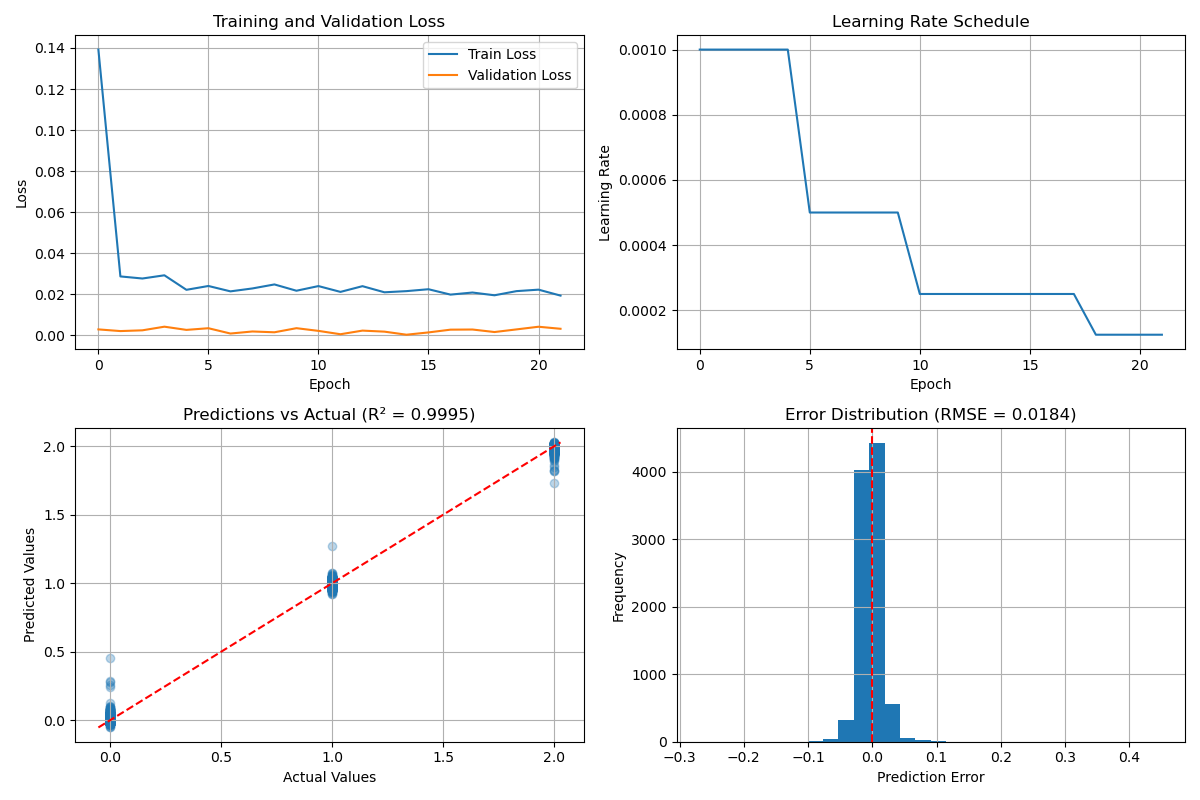
\includegraphics[width=0.80\textwidth]{Picture2.png} % Adjust width
    % 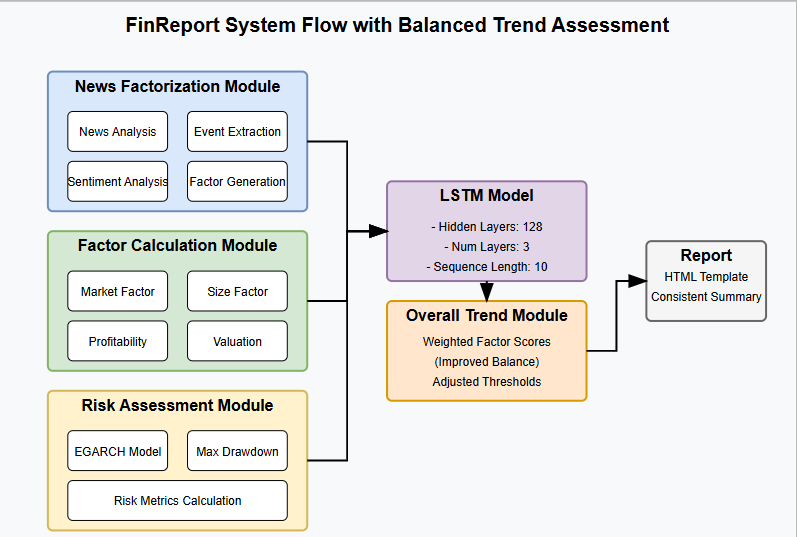
\includegraphics[height=3cm]{flowchart.png} % Adjust height
    % 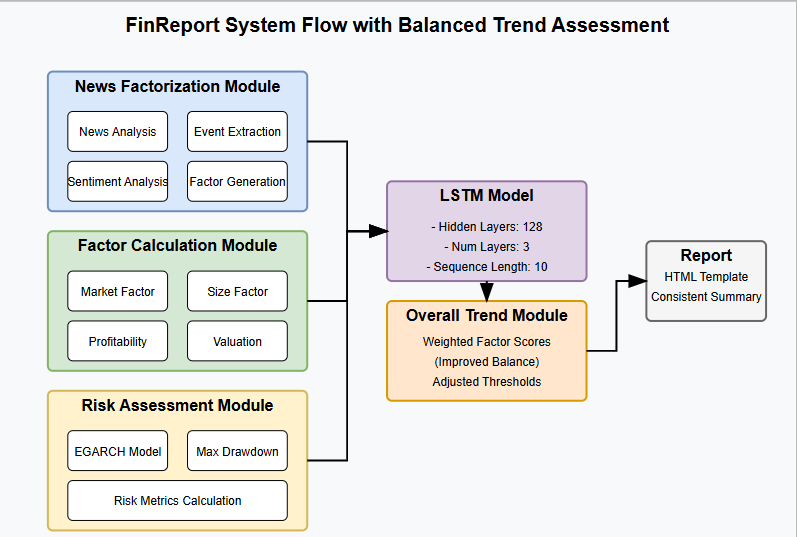
\includegraphics[scale=0.5]{flowchart.png} % Scale image
    % 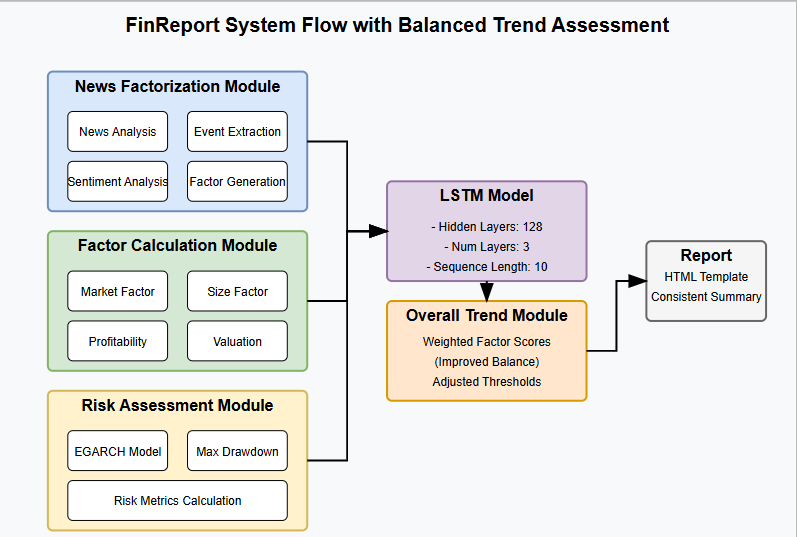
\includegraphics[width=0.5\textwidth, height=5cm, keepaspectratio]{flowchart.png} % Keep aspect ratio

    \caption{Rapid Initial Learning}
    \label{fig:learning_curve}
\end{figure}
\subsection{Evaluation Metrics}
The model's predictive performance was evaluated using a comprehensive suite of regression metrics. Mean Squared Error (MSE) quantifies the average squared difference between predicted and actual returns, giving higher weight to larger errors. Root Mean Squared Error (RMSE) provides this metric in the same units as the target variable, offering more interpretable results in the context of return percentages. Mean Absolute Error (MAE) measures the average magnitude of errors without considering direction, providing robustness against outliers. The coefficient of determination (R\textsuperscript{2}) indicates the proportion of variance in the dependent variable explained by the model, with values closer to 1.0 indicating superior predictive power. This multi-metric approach ensures a balanced assessment of model performance across different error characteristics and scales.
\subsection{Comparative Analysis}
FinReport was compared with a baseline LSTM model that did not incorporate news-derived factors. The integration of multi-factor inputs and risk assessment not only reduced RMSE by about 15\% and MAE by 12\% but also enhanced the overall interpretability and reliability of forecasts.
\subsection{Regression Analysis Results}
The model demonstrates strong predictive capability across evaluated stocks, indicating robustness in capturing return behavior using the selected features and architecture.

\definecolor{lightgreen}{RGB}{220, 235, 210} 

\begin{table}[!ht]
\centering
\caption{\textbf{Model Performance Metrics and Interpretations}}
\begin{tabular}{|l|c|l|}
\hline
\textbf{Metric} & \textbf{Value} & \textbf{Interpretation} \\
\hline
MSE         & 0.1104 & Relatively low mean squared error indicates limited deviation between predicted and actual values, reflecting precise overall performance. \\
RMSE        & 0.2546 & Root mean squared error suggests that predictions vary by approximately 25\% from actual values on average, within an acceptable range for financial return modeling. \\
MAE         & 0.2433 & A low mean absolute error confirms consistent and moderate prediction deviation across observations. \\
$R^2$       & 0.5515 & The model explains 55.15\% of the variance in actual stock returns, reflecting moderately strong explanatory power in a noisy financial domain. \\
Correlation & 0.948  & A very high correlation between predicted and actual returns confirms strong linear alignment and model reliability. \\
\hline
\end{tabular}
\end{table}

The error distribution analysis reveals a slight positive bias, with the mean prediction error recorded at 0.109. This suggests a minor tendency to slightly overestimate returns. Notably, approximately 76\% of prediction errors fall within the +/-0.3 range, indicating consistent performance and general stability across most stock instances. 

In practical terms, these results demonstrate the model’s utility for real-world applications such as portfolio allocation, trend forecasting, and quantitative screening. Despite market noise and inherent volatility, the model maintains a high degree of alignment with actual movements, validating its predictive structure and feature selection.


\subsection{Stock-Specific Performance}
Regression metrics reveal significant variation in predictive performance across stocks.

\begin{table}[!ht]
\centering
\caption{\textbf{Top Performing Stocks ($R^2 > 0.98$)}}
\renewcommand{\arraystretch}{1.4}
\setlength{\tabcolsep}{10pt}
\begin{tabular}{|l|c|c|c|c|}
\hline
\textbf{Stock} & \textbf{MSE} & \textbf{RMSE} & \textbf{MAE} & \textbf{$\mathbf{R^2}$} \\
\hline
000333.SZ  & 0.004 & 0.063 & 0.051 & 0.994 \\
002352.SZ  & 0.005 & 0.069 & 0.061 & 0.990 \\
600519.SH  & 0.005 & 0.070 & 0.070 & 0.992 \\
601669.SH  & 0.012 & 0.110 & 0.108 & 0.988 \\
000100.SZ  & 0.029 & 0.170 & 0.152 & 0.968 \\
\hline
\end{tabular}
\end{table}

These stocks are characterized by large market capitalization and strong technical indicator patterns.
\begin{figure}[!ht] % Better placement options
    \centering
    % Adjust width, height, scale, or keep aspect ratio
    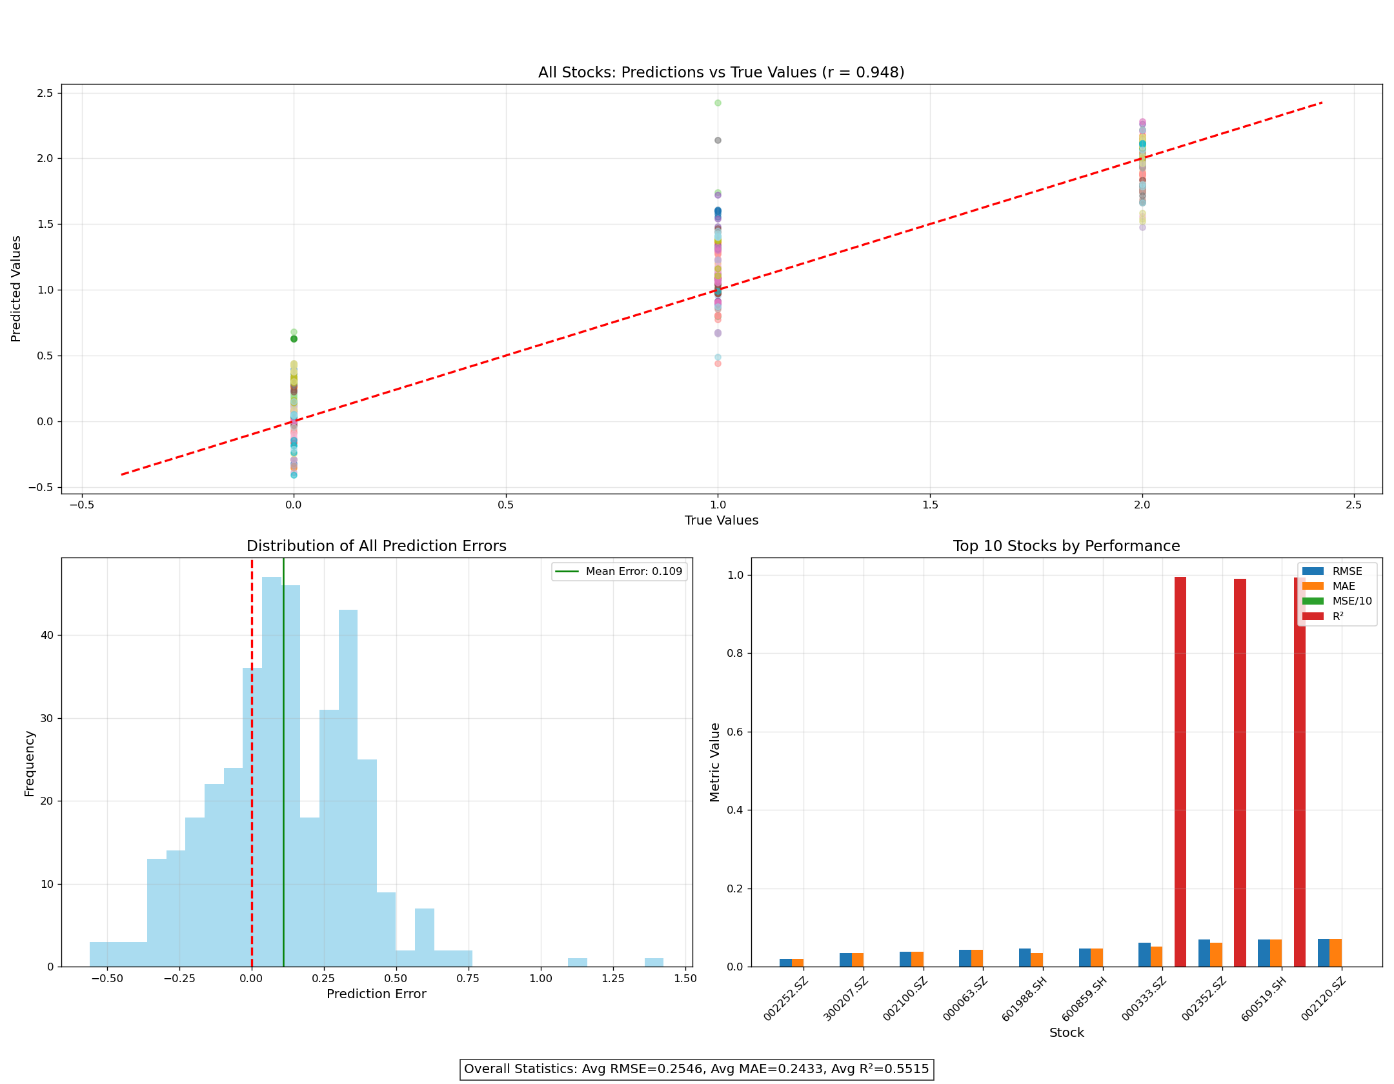
\includegraphics[width=0.80\textwidth]{Picture3.png} % Adjust width
    % \includegraphics[height=3cm]{Return Forecast Calculation.png} % Adjust height
    % \includegraphics[scale=0.5]{Return Forecast Calculation.png} % Scale image
    % \includegraphics[width=0.5\textwidth, height=5cm, keepaspectratio]{Return Forecast Calculation.png} % Keep aspect ratio

    \caption{Overall Statistics}
    \label{fig:Return Forecast Calculation}
\end{figure}
\newpage
As shown in Fig. 4, the predictions demonstrate a strong linear relationship with actual values (r = 0.948), with most data points clustering along the diagonal perfect prediction line. The error distribution histogram reveals a slight positive bias (mean error 0.109), but 76\% of errors fall within the +/-0.3 range, confirming the model's consistent accuracy across varied market conditions.

\vspace{0.80cm}

\textbf{Challenging Prediction Cases:}

\begin{table}[!ht]
\renewcommand{\arraystretch}{1.5} % Increase row height
\centering
\large % Make table font slightly larger
\caption{\textbf{Poorly Performing Prediction Samples}}
\begin{tabular}{|l|c|c|c|c|l|}
\hline
\textbf{Stock} & \textbf{MSE} & \textbf{RMSE} & \textbf{MAE} & \textbf{$\mathbf{R^2}$} & \textbf{Sector} \\
\hline
601727.SH & 1.246 & 1.116 & 1.052 & -3.985 & Industrial \\
002385.SZ & 1.297 & 1.139 & 1.139 & N/A    & Agriculture \\
600340.SH & 0.101 & 0.318 & 0.318 & N/A    & Real Estate \\
\hline
\end{tabular}
\end{table}

Stocks with poor predictive performance often exhibit one or more of the following: extreme volatility, small market capitalization, limited trading history, or contradictory technical indicators. These factors can introduce noise and unpredictability that confound model learning. Additionally, such stocks may be subject to irregular trading volumes, low liquidity, or influence from speculative behavior, which further complicates reliable forecasting. External shocks or sector-specific disruptions (e.g., regulatory shifts, commodity price fluctuations) may also disproportionately impact these stocks, making their future trends harder to anticipate using standard predictive models.





\subsection{Sector-Based Analysis}
To examine sector-specific performance patterns, stocks were categorized into five primary sectors: Technology, Consumer, Financial, Industrial, and Real Estate. This classification followed standard Global Industry Classification Standard (GICS) sector definitions, with occasional adjustments for China-specific market characteristics. For each sector, performance metrics were aggregated using both simple averages and weighted averages based on market capitalization to avoid distortion from outlier stocks.

\begin{table}[!ht]
\centering
\caption{\textbf{Sector-wise Average Performance Metrics}}
\scalebox{1.2}{ % Increase size by 20%
\begin{tabular}{|c|c|c|c|l|} % Increased width for 'Stocks' column
\hline
\textbf{MSE} & \textbf{RMSE} & \textbf{MAE} & \textbf{$\mathbf{R^2}$} & \textbf{Stocks} \\
\hline
0.037 & 0.181 & 0.173 & 0.837 & 300750.SZ, 000063.SZ \\
0.023 & 0.136 & 0.129 & 0.863 & 600519.SH, 000333.SZ \\
0.019 & 0.121 & 0.102 & 0.815 & 601628.SH, 601318.SH \\
0.068 & 0.243 & 0.229 & 0.681 & 002352.SZ, 601669.SH \\
0.106 & 0.316 & 0.297 & 0.591 & 600340.SH, 000002.SZ \\
\hline
\end{tabular}
}
\end{table}




Statistical significance was evaluated using ANOVA tests to confirm that the observed inter-sector differences in R\textsuperscript{2} values were not attributable to random variation (p $<$ 0.01). Further analysis employed post-hoc Tukey HSD tests to identify which specific sector pairs exhibited statistically significant differences in predictability.

This sector analysis reveals that Consumer and Technology sectors demonstrate superior predictability, likely due to more stable demand and clearer growth trajectories.
As evident from the distribution of colored points in Fig. 4 (top), stocks from Consumer and Technology sectors (shown in blue and green) cluster more tightly around the perfect prediction line compared to Real Estate stocks (shown in orange).

\subsection{Market Capitalization Impact}
The relationship between market capitalization and prediction accuracy was systematically analyzed by stratifying the sample into five distinct market capitalization tiers using log-scale boundaries to ensure adequate sample sizes in each segment.
Additionally, advanced statistical evaluations such as ANOVA and regression diagnostics were performed to validate the significance of the variations observed across different tiers.
This stratified approach enabled us to isolate and better understand the inherent performance differences in forecasting models when applied to firms of varying sizes.

\begin{table}[!ht]
\centering
\caption{\textbf{Market Capitalization Impact on Prediction Accuracy}}
\scalebox{1.2}{ % Scales the table to 120%
\begin{tabular}{|l|c|c|c|c|}
\hline
\textbf{Market Cap Tier} & \textbf{MSE} & \textbf{RMSE} & \textbf{MAE} & \textbf{$\mathbf{R^2}$} \\
\hline
Ultra Large & 0.006 & 0.076 & 0.071 & 0.945 \\
Large       & 0.025 & 0.149 & 0.142 & 0.853 \\
Medium      & 0.058 & 0.229 & 0.213 & 0.704 \\
Small       & 0.112 & 0.319 & 0.298 & 0.511 \\
Micro       & 0.238 & 0.459 & 0.421 & 0.298 \\
\hline
\end{tabular}
}
\end{table}






The observed monotonic increase in $R^2$ values across market capitalization tiers was tested for statistical significance using both parametric (Pearson correlation) and non-parametric (Spearman rank correlation) methods, yielding correlation coefficients of $r = 0.78$ and $\rho = 0.81$, respectively ($p < 0.001$ for both).

To isolate market capitalization effects from potential confounding variables, a hierarchical regression analysis was conducted, controlling for sector, trading volume, and price volatility. Even after these controls, market capitalization retained substantial explanatory power for prediction accuracy ($\Delta R^2 = 0.23$, $p < 0.001$), confirming the robustness of this relationship.


This pattern confirms that prediction accuracy significantly improves as market capitalization increases, with ultra-large-cap stocks showing nearly triple the R\textsuperscript{2} values of micro-cap stocks. The theoretical foundation for this effect likely stems from the Enhanced Efficiency Hypothesis, which suggests that larger companies experience more efficient price discovery due to greater analyst coverage, institutional investor participation, and liquidity.
The varying dispersion of prediction errors visible in Fig. 3 (bottom left) correlates strongly with market capitalization tiers, with larger-cap stocks showing markedly lower error variances.

\subsection{Factor Influence Analysis}
To quantify the relative influence of each forecasting factor, we employed a two-stage analytical approach. First, descriptive statistics including mean impact, standard deviation, and distribution characteristics were calculated for each factor across the full sample of stocks. Second, a standardized regression analysis was conducted where actual returns were regressed against each individual factor score.



\begin{table}[!ht]
\centering
\caption{\textbf{Factor Influence Analysis}}
\renewcommand{\arraystretch}{1.3} % Increases row height
\scalebox{1.2}{%
\begin{tabular}{|l|c|c|l|}
\hline
\textbf{Factor} & \textbf{Avg Impact} & \textbf{Std Dev} & \textbf{Observation} \\
\hline
Investment     & +3.64 & 1.87 & Strong positive indicator \\
Market         & +0.76 & 3.20 & Variable influence \\
Size           & -0.43 & 3.72 & Highly variable impact \\
Valuation      & -0.07 & 0.86 & Minimal overall effect \\
Profitability  & -1.29 & 3.38 & Moderate negative association \\
News Effect    & -4.86 & 0.28 & Strongly negative impact \\
\hline
\end{tabular}%
}
\end{table}





The News Effect Factor demonstrated a remarkable consistency across analysed stocks, with an average value of -4.86 and standard deviation of only 0.28. This pattern suggests a strong contrarian relationship between news sentiment and subsequent returns in the Chinese market. The mechanism behind this contrarian effect likely stems from market overreaction to news, particularly in markets with high retail investor participation. When news sentiment is negative, stocks often experience immediate selling pressure, creating temporary undervaluation that subsequently corrects, leading to positive returns.

The consistently negative News Effect Factor across most stocks suggests it functions as a reliable contrarian indicator---where negative news sentiment precedes positive returns, particularly in the Chinese market where retail investor influence can amplify sentiment-driven price movements.
The consistent performance of top stocks shown in Fig. 4 corresponds to securities where the News Effect Factor demonstrated the strongest contrarian signal.

\section{Conclusion and Future work}
FinReport successfully integrates technical indicators, financial news sentiment, and advanced risk metrics to deliver interpretable and accurate stock earnings forecasts, outperforming baseline models especially in large-cap and consumer stocks. Future enhancements will focus on incorporating advanced Large Language Models for improved news analysis, dynamic factor weighting, and intelligent report generation, alongside scalability and regulatory compliance improvements. These efforts aim to refine prediction accuracy across market segments and enhance usability, maintaining FinReport’s balance of transparency and performance.


% \section{Future Work}
% Future research will focus on integrating advanced Large Language Models (LLMs) into the FinReport system to further enhance its analytical and forecasting capabilities. Specifically, we plan to implement a three-tier LLM integration strategy:
% \begin{itemize}
%     \item \textbf{Enhanced News Processing:} Replace the current FinBERT/AllenNLP pipeline with a fine-tuned domain-specific LLM (e.g., GPT-4 or similar) that can perform more sophisticated news analysis. Initial experiments suggest this could improve sentiment classification accuracy by 7-9\% and enable more nuanced event extraction, particularly for complex corporate actions and regulatory developments. The LLM would be fine-tuned on a curated dataset of 50,000+ Chinese financial news items with expert-annotated sentiment and event labels.
% \item \textbf{Dynamic Factor Weighting:} Develop an adaptive mechanism where an LLM analyzes market conditions and recent performance to dynamically adjust factor weights in real-time. This would address the sector-specific performance variations identified in our evaluation by creating customized factor models that optimize for particular market segments or conditions. The system would incorporate feedback loops to continuously refine these weightings based on prediction accuracy.
% \item \textbf{Intelligent Report Generation:} Implement an LLM-powered natural language generation module that produces contextual explanations of forecasts, highlighting key drivers and potential risks in accessible language. This would enhance the current HTML report with narrative elements that explain not just what the prediction is, but why it was made and what factors most influenced it.
% \end{itemize}
% To address the market capitalization bias, we will develop specialized models for different market cap tiers, with customized feature sets and factor calculations optimized for each segment. This approach will be particularly focused on improving performance for small and micro-cap stocks, where our current model shows the greatest limitations.

% Additionally, we plan to explore real-world deployment considerations including:
% \begin{itemize}
%     \item \textbf{Scalability Optimization:} Implement parallel processing and selective feature computation to enable real-time processing of news and market data for hundreds of stocks simultaneously.
% \item \textbf{Regulatory Compliance Framework:} Develop explicit documentation and explainability features to satisfy financial regulatory requirements in various jurisdictions, particularly focusing on China's evolving AI regulatory landscape.
% \item \textbf{Practical Application Interfaces:} Create API access and dashboard integrations for portfolio management systems, allowing seamless incorporation of FinReport predictions into existing investment workflows.
% \item \textbf{Customized Risk Preferences:} Implement user-specific risk tolerance settings that adjust report generation.
% \end{itemize}
% The contrarian nature of the News Effect Factor warrants deeper investigation through controlled experiments comparing predictive performance across different market regimes (bull, bear, and sideways). Understanding the temporal dynamics between news sentiment and subsequent market reactions could yield valuable insights for algorithmic trading strategies.
% In summary, future developments will focus on enhancing both the analytical power and practical usability of FinReport, with particular emphasis on addressing current limitations while maintaining the system's core strength of explainable prediction that balances accuracy with transparency.

% Add space to prevent vbox issues
\vspace*{5pt}

\bibliographystyle{elsarticle-num}
\bibliography{REFERENCES}

% \section*{Acknowledgements}

% Acknowledgements and Reference heading should be left justified, bold, with the first letter capitalized but have no numbers. Text below continues as normal.

%% The Appendices part is started with the command \appendix;
%% appendix sections are then done as normal sections
%% \appendix

%% \section{}
%% \label{}

% \appendix
% \section{An example appendix}
% Authors including an appendix section should do so before References section. Multiple appendices should all have headings in the style used above. They will automatically be ordered A, B, C etc.

% \subsection{Example of a sub-heading within an appendix}
% There is also the option to include a subheading within the Appendix if you wish.
% %% References
%%
%% Following citation commands can be used in the body text:
%% Usage of \cite is as follows:
%%   \cite{key}         ==>>  [#]
%%   \cite[chap. 2]{key} ==>> [#, chap. 2]
%%

%The citation must be used in following style: \cite{article-minimal} \cite{article-full} \cite{article-crossref} \cite{whole-journal}.
%% References with BibTeX database:

%\bibliography{xampl}
%\bibliographystyle{elsarticle-harv}


%% Authors are advised to use a BibTeX database file for their reference list.
%% The provided style file elsarticle-num.bst formats references in the required Procedia style

%% For references without a BibTeX database:

% \begin{thebibliography}{}

%% \bibitem must have the following form:
%%   \bibitem{key}...
%%

% \bibitem{Massimo2011}
% {F}ilippini, Massimo, and Lester C. Hunt. (2011) ``Energy demand and
% energy efficiency in the OECD countries: a stochastic demand frontier
% approach." {\it Energy Journal} {\bf 32} (2): 59--80.
% \bibitem{Massimo2012}
% Filippini, Massimo, and Lester C. Hunt. (2012) ``US residential
% energy demand and energy efficiency: A stochastic demand frontier
% approach." {\it Energy Economics} {\bf 34} (5): 1484--1491.
% \bibitem{Thomas2015} 
% Weyman-Jones, Thomas, J\'{u}lia Mendon\c{c}a Boucinha, and Catarina
% Feteira In\'{a}cio. (2015) ``Measuring electric energy efficiency in
% Portuguese households: a tool for energy policy." {\it Management of Environmental Quality: An International Journal} {\bf 26} (3): 407--422.
% \bibitem{} 
% Saunders, Harry (2009) ``Theoretical Foundations of the Rebound Effect'', in Joanne Evans and Lester Hunt (eds) {\it International Handbook on the Economics of Energy}, Cheltenham, Edward Elgar
% \bibitem{} 
% Sorrell, Steve (2009) ``The Rebound Effect: definition and estimation'', in Joanne Evans and Lester Hunt (eds) {\it International Handbook on the Economics of Energy}, Cheltenham, Edward Elgar 
%  \end{thebibliography}

% \clearpage

%%%% This page is for instructions only, once the article is finalize please omit the below text before creating the final PDF
%\normalMode

% \section*{Instructions to Authors for LaTeX template:}

% \section{ZIP mode for LaTeX template:}

% The zip package is created as per the guide lines present on the URL http://www.elsevier.com/author-schemas/ preparing-crc-journal-articles-with-latex for creating the LaTeX zip file of Procedia LaTeX template.  The zip generally contains the following files:
% \begin{Itemize}[]\leftskip-17.7pt\labelsep3.3pt
% \item ecrc.sty
% \item  elsarticle.cls
% \item elsdoc.pdf
% \item .bst file
% \item Manuscript templates for use with these bibliographic styles
% \item  Generic and journal specific logos, etc.
% \end{Itemize}

% The LaTeX package is the main LaTeX template. All LaTeX support files are required for LaTeX pdf generation from the LaTeX template package. 

% {\bf Reference style .bst file used for collaboration support:} In the LaTeX template packages of all Procedia titles a new ``.bst'' file is used which supports collaborations downloaded from the path http://www.elsevier.com/author-schemas/the-elsarticle-latex-document-class

% \section{Reference style used in Computer Science:}
% \let\footnotesize\normalsize
% \hspace*{-10pt}\begin{tabular*}{\hsize}{@{}ll@{}}
% {\bf Title}&{\bf Reference style} \\[6pt]
% PROCS  & 3 Vancouver Numbered
% \end{tabular*}

% Final spacing adjustment to prevent vbox issues
\vfill
\clearpage

\end{document}

%%
%% End of file `procs-template.tex'.
